\documentclass[]{book}

%These tell TeX which packages to use.
\usepackage{array,epsfig}
\usepackage{amsmath}
\usepackage{amsfonts}
\usepackage{amssymb}
\usepackage{amsxtra}
\usepackage{amsthm}
\usepackage{mathrsfs}
\usepackage{color}
\usepackage{graphicx}
\usepackage{float}

%Algorithm packages
\usepackage{algorithm}  
\usepackage{algpseudocode}  
\usepackage{amsmath}  
\renewcommand{\algorithmicrequire}{\textbf{Input:}}  % Use Input in the format of Algorithm  
\renewcommand{\algorithmicensure}{\textbf{Output:}} % Use Output in the format of Algorithm  
%Here I define some theorem styles and shortcut commands for symbols I use often
\theoremstyle{definition}
\newtheorem{defn}{Definition}
\newtheorem{thm}{Theorem}
\newtheorem{cor}{Corollary}
\newtheorem*{rmk}{Remark}
\newtheorem{lem}{Lemma}
\newtheorem*{joke}{Joke}
\newtheorem{ex}{Example}
\newtheorem*{soln}{Solution}
\newtheorem{prop}{Proposition}

\newcommand{\lra}{\longrightarrow}
\newcommand{\ra}{\rightarrow}
\newcommand{\surj}{\twoheadrightarrow}
\newcommand{\graph}{\mathrm{graph}}
\newcommand{\bb}[1]{\mathbb{#1}}
\newcommand{\Z}{\bb{Z}}
\newcommand{\Q}{\bb{Q}}
\newcommand{\R}{\bb{R}}
\newcommand{\C}{\bb{C}}
\newcommand{\N}{\bb{N}}
\newcommand{\M}{\mathbf{M}}
\newcommand{\m}{\mathbf{m}}
\newcommand{\MM}{\mathscr{M}}
\newcommand{\HH}{\mathscr{H}}
\newcommand{\Om}{\Omega}
\newcommand{\Ho}{\in\HH(\Om)}
\newcommand{\bd}{\partial}
\newcommand{\del}{\partial}
\newcommand{\bardel}{\overline\partial}
\newcommand{\textdf}[1]{\textbf{\textsf{#1}}\index{#1}}
\newcommand{\img}{\mathrm{img}}
\newcommand{\ip}[2]{\left\langle{#1},{#2}\right\rangle}
\newcommand{\inter}[1]{\mathrm{int}{#1}}
\newcommand{\exter}[1]{\mathrm{ext}{#1}}
\newcommand{\cl}[1]{\mathrm{cl}{#1}}
\newcommand{\ds}{\displaystyle}
\newcommand{\vol}{\mathrm{vol}}
\newcommand{\cnt}{\mathrm{ct}}
\newcommand{\osc}{\mathrm{osc}}
\newcommand{\LL}{\mathbf{L}}
\newcommand{\UU}{\mathbf{U}}
\newcommand{\support}{\mathrm{support}}
\newcommand{\AND}{\;\wedge\;}
\newcommand{\OR}{\;\vee\;}
\newcommand{\Oset}{\varnothing}
\newcommand{\st}{\ni}
\newcommand{\wh}{\widehat}

%Pagination stuff.
\setlength{\topmargin}{-.3 in}
\setlength{\oddsidemargin}{0in}
\setlength{\evensidemargin}{0in}
\setlength{\textheight}{9.in}
\setlength{\textwidth}{6.5in}
\pagestyle{empty}



\begin{document}


\begin{center}
{\Large COMP 540 \hspace{0.5cm} HW 1}\\
\textbf{Peiguang Wang, Xinran Zhou}\\ %You should put your name here
Due: 1/18/2018 %You should write the date here.
\end{center}

\vspace{0.2 cm}


\subsection*{Part 0: Background refresher}

%% Problem 1
\begin{enumerate}
\item\label{norms}
Generate different distributions from uniform distribution:
\begin{enumerate}
	\item	Plot the histogram of a categorical distribution with probabilities [0.2,0.4,0.3,0.1].
	\begin{center}
		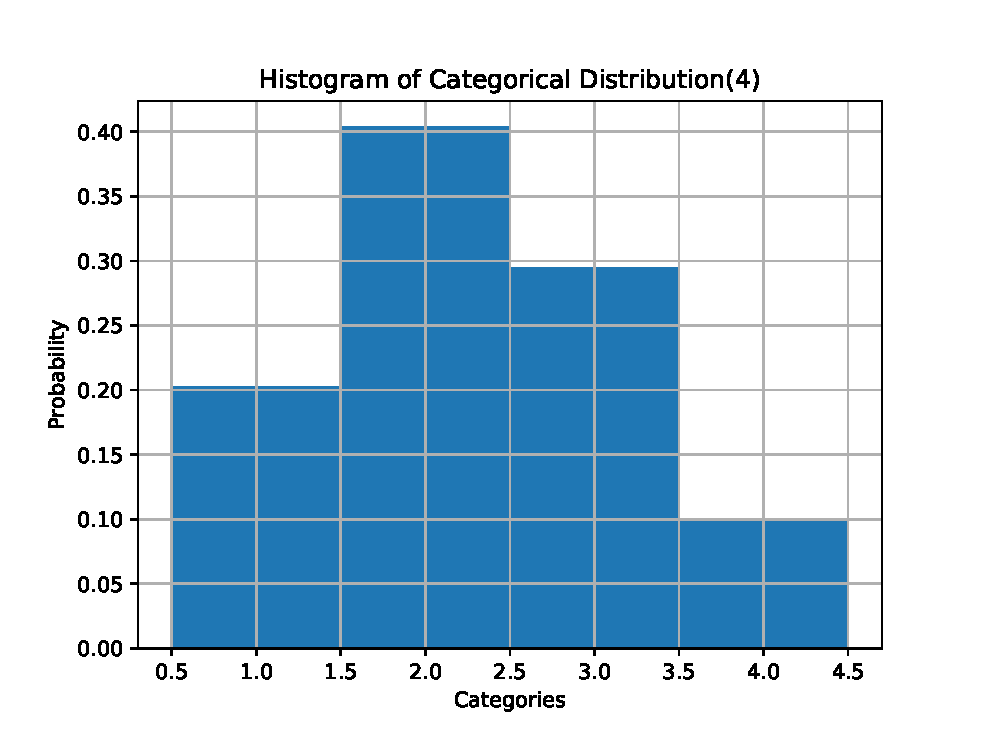
\includegraphics[height=7cm]{cd}
	\end{center}
	\item	Plot the univariate normal distribution with mean of 10 and standard deviation of 1.
	\begin{center}
		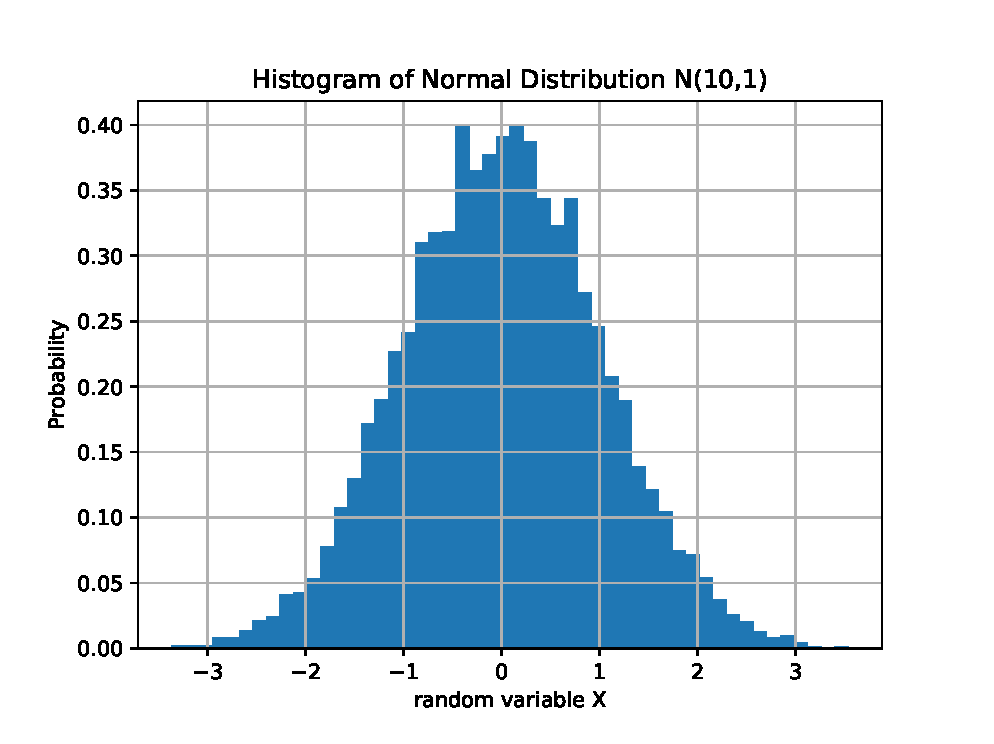
\includegraphics[height=7cm]{und}
	\end{center}
	\item	Produce a scatter plot of the samples for a 2-D Gaussian with mean at [1,1] and a covariance matrix [[1,0.5],[0.5,1]]
	\begin{center}
		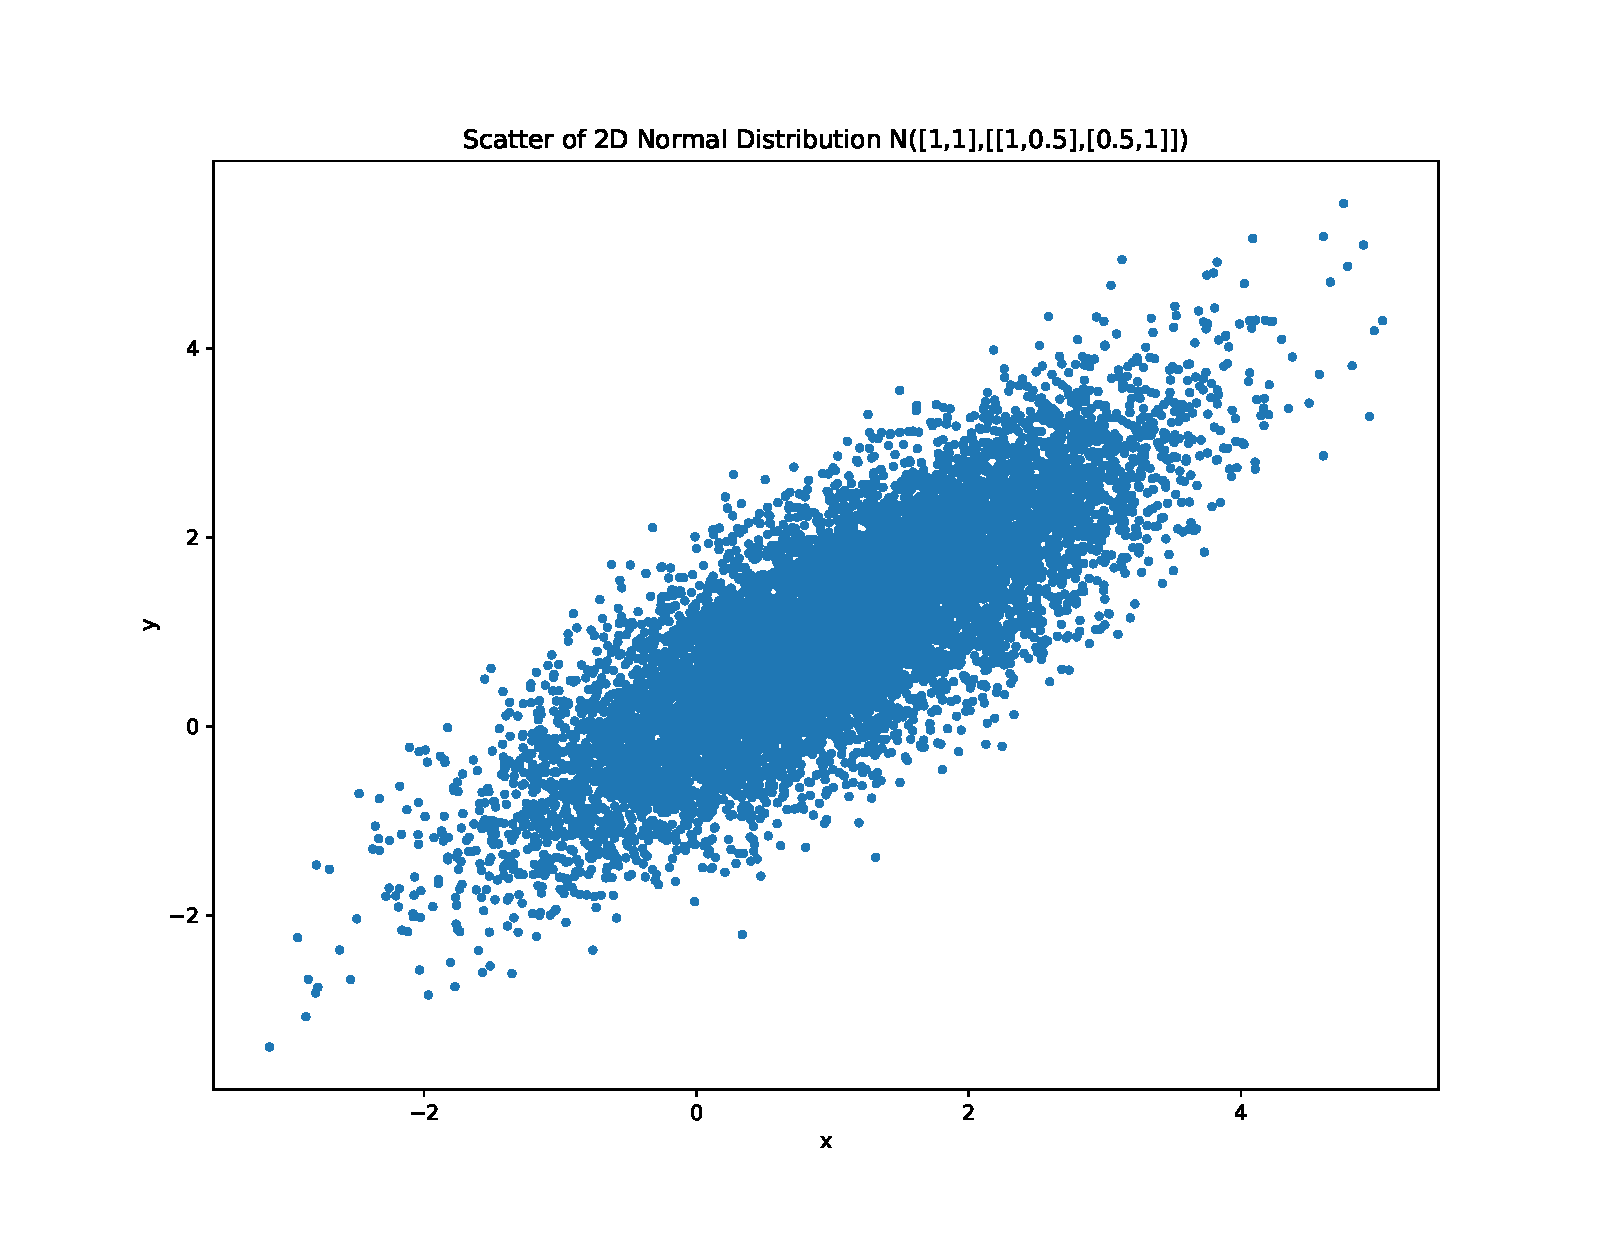
\includegraphics[height=8cm]{mund}
	\end{center}
	\item	Test your mixture sampling code by writing a function that implements an equal weighted mixture of four Gaussians in 2 dimensions, centered at $(\pm 1; \pm 1)$ and having covariance $I$. Estimate the probability that a sample from this distribution lies within the unit circle centered at (0.1, 0.2).	
	
	\begin{soln}
		The Probability that falls in unit circle with center at (0.1,0.2) is 0.1815.
	\end{soln}

\end{enumerate}

%% Problem 2
\item	Prove that the sum of two independent Poisson random variables is also a Poisson random variable.
\begin{proof}
	The characteristic function of a Poisson random variable is
	$$\varPhi _1(u) = e^{\lambda _1 (e^{iu}-1)}$$
	
	Let $X_1$ and $X_2$ denote two independent Poisson random variables. Let $X=X_1+X_2$
	
	Let $\varPhi _1(u)$ and $\varPhi _2(u)$ denote the characteristic functions of $X_1$ and $X_2$:
	$$\varPhi _1(u) = e^{\lambda _1 (e^{iu}-1)}$$
	$$\varPhi _2(u) = e^{\lambda _2 (e^{iu}-1)}$$
	
	Let $\varPhi (u)$ denote the characteristic functions of $X$. Since $X=X_1 + X_2$, we have:
	$$\varPhi (u) = \varPhi _1(u) \varPhi _2(u)=e^{\lambda _1 (e^{iu}-1)}e^{\lambda _2 (e^{iu}-1)}$$
	Simplify the equation above,
	$$\varPhi (u) = e^{(\lambda _1 + \lambda _2) ( \frac{\lambda_1}{\lambda_1 + \lambda_2}e^{iu} + \frac{\lambda_2}{\lambda_1 + \lambda_2}e^{iu}) - 1 }. $$
	That is
	$$\varPhi (u) = e^{(\lambda_1 + \lambda_2)  (e^{iu}-1)}. $$
	Comparing with the characteristic function of Poisson distribution, we can see that X is also a Poisson random variable.
\end{proof}

%% Problem 3
\item	Let $X_0$ and $X_1$ be continuous random variables. Show that if
	$$P(X_0=x_0) = \alpha_0	e^{-\frac{(x_0-\mu_0)^2}{2 \sigma_0^2}}$$
	$$P(X_1=x_1|X_0=x_0) = \alpha	e^{-\frac{(x_1-x_0)^2}{2 \sigma^2}}$$
there exists $\alpha_1$, $\mu_1$ and $\sigma_1$ such that
$$P(X_1=x_1) = \alpha_1	e^{-\frac{(x_1-\mu_1)^2}{2 \sigma_1^2}}$$	
Write down expressions for these quantities in terms of $\alpha_0$, $\alpha$, $\mu_0$, $\sigma_0$ and $\sigma$.

\begin{soln}
	If X,Y are both Gaussian random variable, then
	$$Y|X=x\sim N\left(\mu_Y+\rho \dfrac{\sigma_Y}{\sigma_X}(X-\mu_X),\quad \sigma^2_Y(1-\rho^2)\right)$$ 
	where $\mu_X$, $\mu_Y$ are mean of $X$ and $Y$; $\sigma_X^2$, $\sigma_Y^2$ are variance of $X$ and $Y$; $\rho$ is the correlation coefficient between $X$ and $Y$.
	
	According to the problem, $X_0$, $X_1$ and $X_1 | X_0$ are all Gaussian. So we have the following equations:
	$$ \left\{
	\begin{aligned}
	\mu_1 + \rho \frac{\sigma_1}{\sigma_0}(x_0 - \mu_0) & =  x_0 ,   for \; all \; x_0 \\ 
	\sigma_1^2  (1-\rho^2) & =  \sigma^2 
	\end{aligned} 
	\right.
	$$

	Solve the equation, then $\sigma_1^2 = \sigma^2 + \sigma_0^2$, $\mu_1 = -\mu_0$. 
	And since $\alpha_1 = \frac{1}{\sqrt{2 \pi} \sigma_1}$, we have 
	$$\alpha_1 = \sqrt{ \frac{1}{(1/\alpha)^2 + (1/\alpha_0)^2}  } $$.
	
\end{soln}

%% Problem 4
\item	Find the eigenvalues and eigenvectors of the following 2 $\times$ 2 matrix $A$.
$$A = \left({
\begin{matrix}

13 & 5 \\ 
2 & 4
\end{matrix}
}\right) $$

\begin{soln}
	Let $\lambda$ and \boldmath $x$ \unboldmath denote the eigenvalue and eigenvector of A. According to the definition of eigenvalue,
	$$A \boldsymbol{x} = \lambda \boldsymbol{x} $$
	Solve the equation to get eigenvalues
	$$ |A-\lambda I| = 0 $$
	That is,
	$$\lambda ^2 -14\lambda +42 = 0$$
	A has two eigenvalues: $\lambda_1 = 14$, $\lambda_2 = 3$.
	
	When $\lambda$ = 14,
	$$(A- \lambda I) \boldsymbol{x}  = \left( {\begin{matrix}
	-1 & 5 \\ 
	2 & -10
	\end{matrix} }\right) \boldsymbol{x} = 0 $$
	$$\boldsymbol{x} = \left({\begin{matrix}
		5 & 1
		\end{matrix} }\right) ^ T $$
	When $\lambda$ = 3,
	$$(A- \lambda I) \boldsymbol{x}  = \left( {\begin{matrix}
		10 & 5 \\ 
		2 & 1
		\end{matrix} }\right) \boldsymbol{x} = 0 $$
	$$\boldsymbol{x} = \left({\begin{matrix}
		1 & -2
		\end{matrix} }\right) ^ T $$
	
	In summary, A has two eigenvalues, $\lambda_1 = 14$, $\lambda_2 = 3$. The corresponding eigenvectors are $\boldsymbol{x_1} = \left({\begin{matrix}
		5 & 1
		\end{matrix} }\right) ^ T $ and $\boldsymbol{x_2} = \left({\begin{matrix}
		1 & -2
		\end{matrix} }\right) ^ T $.
	
\end{soln}

%% Problem 5
\item	Provide one example for each of the following cases, where A and B are 2 × 2 matrices.
\begin{enumerate}
	\item  $(A + B)^2 \neq A^2 + 2AB + B^2$
	\item  $AB = 0, A \neq 0, B \neq 0$
\end{enumerate}

\begin{soln}
	\begin{enumerate}
		\item one example that satisfies (a) is:
		$$A=\left({\begin{matrix}
			0 & 0 \\ 
			0 & 1
			\end{matrix} }\right), 
		B = \left({\begin{matrix}
			0 & 1 \\ 
			0 & 0
			\end{matrix} }\right)$$
		Calculate left,
		$$left = (A+B)^2 = \left({\begin{matrix}
			0 & 1 \\ 
			0 & 0
			\end{matrix} }\right) \left({\begin{matrix}
			0 & 1 \\ 
			0 & 0
			\end{matrix} }\right) = \left({\begin{matrix}
			0 & 1 \\ 
			0 & 1
			\end{matrix} }\right)$$
		Calculate right,
		$$right = A^2 + 2AB + B^2 = \left({\begin{matrix}
			0 & 0 \\ 
			0 & 1
			\end{matrix} }\right) + \boldsymbol{0} + \boldsymbol{0} = \left({\begin{matrix}
			0 & 0 \\ 
			0 & 1
			\end{matrix} }\right)$$
		And $left \neq right$
		
		\item 	one example that satisfies (b) is:
		$$A=\left({\begin{matrix}
			0 & 0 \\ 
			0 & 1
			\end{matrix} }\right), 
		B = \left({\begin{matrix}
			0 & 1 \\ 
			0 & 0
			\end{matrix} }\right)$$
		where $A\neq 0$, and $B \neq 0$. Calculate $AB$,
		$$AB = \left({\begin{matrix}
			0 & 0 \\ 
			0 & 1
			\end{matrix} }\right) \left({\begin{matrix}
			0 & 1 \\ 
			0 & 0
			\end{matrix} }\right) = \boldsymbol{0} $$		
	\end{enumerate}
\end{soln}

\item Let $u$ denote a real vector normalized to unit length. That is, $u^T u = 1$. Show that
$$A = I - 2 u u^T $$
is orthogonal, i.e., $A^T A = 1$.
\begin{proof}
	Derive from left,
	$$A^T A = (I-2u u^T)^T(I-2u u^T) =(I-2u u^T)(I-2u u^T) = I-2u u^T - 2u u^T + 4 u u^T = I$$
	So $left = right$.	
\end{proof}

\end{enumerate}

%% part1
\subsection*{Part 1: Locally weighted linear regression}
%% part1 problem 1
\begin{enumerate}
	\item Show that $J(\theta)$ can be written in the form
	$$J(\theta)=(X \theta - y)^T W (X \theta - y)$$
	for an appropriate diagonal matrix $W$, where $X$ is the $m \times d$ input matrix and y is a $m \times 1$ vector denoting the associated outputs. State clearly what $W$ is.
\begin{proof}
	We know that $J(\theta)$ can also be written as 
	$$J(\theta)=\frac{1}{2} \sum_{i=1}^{m} w^{(i)} (\theta^T x^{(i)} - y^{(i)})^2$$
	where $x^{(i)}$ is $d \times 1$ vector and $\theta$ is a $d \times 1$ vector. We consider each row of the matrix $X$ as as a $1 \times d$vector $x^i$, so we can write $X = [x^1, x^2, ..., x^m]^T$. So
	$$J(\theta)=(X \theta - y)^T W (X \theta - y)
	=[x^1 \theta - y^1, x^2 \theta - y^2,...,x^m \theta - y^m] W [x^1 \theta - y^1, x^2 \theta - y^2,...,x^m \theta - y^m]^T$$
	So $W$ is a $m \times m$ diagonal matrix
	$$W=\left(\begin{matrix}
	2 w^{(1)} & 0 & 0 & 0 \\ 
		0 & 2 w^{(2)} & 0 & 0 \\ 
		0 & 0 & ... & 0  \\ 
		0 & 0 & 0 & 2 w^{(m)}
	
	\end{matrix}\right)$$ 
\end{proof}
	
%%part 1 problem 2
	\item If all the $w^{(i)}$'s are equal to 1, the normal equation to solve for the parameter $\theta$ is:
	$$X^T X \theta = X^T y$$
	and the value of $\theta$ that minimizes $J(\theta)$ is $(X^T X)^{-1} X^T y$. By computing the derivative of the weighted $J(\theta)$ and setting it equal to zero, generalized the normal equation to the weighted setting and solve for $\theta$ in closed form in terms of $W$, $X$ and $y$.
\begin{proof}
	$$J(\theta)=(X \theta - y)^T W (X \theta - y)=\theta^T X^T W X \theta^T - \theta^T X^T W y - y^T W X \theta + y^T W y$$
	Compute the derivative of $J(\theta)$
	$$\frac{\partial{J(\theta)}}{\partial(\theta)}=2 X^T W X \theta -X^T W y - X^T W^T y$$
	Since $W$ is a diagonal matirx $W = W^T$, the equation can be written as
	$$\frac{\partial{J(\theta)}}{\partial(\theta)} = 2 X^T W X \theta -2 X^T W y$$
	By setting it equal to zero, we can find the value of $\theta$ that minimizes $J(\theta)$, the equation is :
	$$X^T W X \theta = X^T W y $$
	So the value of $\theta$ in form in terms of $W$, $X$ and $y$ is $(X^T W X)^{-1} X^T W y$.
\end{proof} 

%% part 1 problem 3
	\item To predict the target value for an input vector $x$, one choice for the weighting function $w^{(i)}$ is:
	$$w^{(i)}= \exp({-\frac{(x -x^{(i)})^T (x-x^{(i)})}{2 \tau^2}})$$
	%% big 
	Points near $x$ are weighted more heavily than points far away from $x$. The parameter $\tau$ is a band width defining the sphere of influence around $x$. Note how the weights are defined by the input $x$. Write down an algorithm for calculating $\theta$ by batch gradient descent for locally weighted linear regression. Is locally weighted linear regression a parametric or a non-parametric method?
	
	\begin{soln}
		Algorithm to calculate $\theta$ is shown below. 
		
		{\centering
			\begin{minipage}{.75\linewidth}
				\begin{algorithm}[H]
					\caption{Weighted linear regression using batch gradient descent}  
					\begin{algorithmic}[1]  
						\State Calculate $W$ using $w^{(i)}= \exp({-\frac{(x -x^{(i)})^T (x-x^{(i)})}{2 \tau^2}})$;  
						\State Set learnign rate $\alpha$;
						
						\For{enough iterations}
						\State Update $\theta$ where $\theta_j = \theta_j - \alpha \sum_{i = 1}^{m}w^{(i)}(\theta^Tx^{(i)}-y^{(i)})x_j$ 
						\EndFor 
						\\  
						\Return $\theta$;  
					\end{algorithmic}  
				\end{algorithm}   
			\end{minipage}
		}
		  
		Because it uses data points when predicting, it is a non-parametric method.
	\end{soln}
\end{enumerate}

%%part 2 
\subsection*{Part 2: Properties of the linear regression estimator}

\begin{enumerate}
%% part 2 problem 1
	\item Show that $E[\theta]= \theta^*$ for the least squares estimator.
	
\begin{proof}
	In part 1 problem 2, we can get thee value of $\theta$ given the normal equation $X^T X \theta = X^T y$ is 
	$$\theta = (X^T X)^{-1} X^T y$$
	The date comes from the linear model:
	$$y^{(i)} = \theta^T x^{(i)} + \epsilon^{(i)} $$
	the expectation of $\theta$ is
	 \begin{equation*}
		\begin{split}
		E[\theta] &= E[(X^T X)^{-1} X^T y]\\
				 &= E[(X^T X)^{-1} X^T (X\theta^* + \epsilon)]\\
				 &=E[(X^T X)^{-1} (X^T X \theta^* +X^T \epsilon)]\\
				 &=E[(X^T X)^{-1}X^T X\theta^* + (X^T X)^{-1} X^T \epsilon]\\
				 &=E[\theta^*] +E[(X^T X)^{-1} X^T \epsilon]
		\end{split}
		\end{equation*}
	since each $\epsilon^{(i)}$is an independent random variable drawn from a normal distribution with zero mean and variance $\sigma^2$ and $\theta^*$ is a true parameter that has certain value. Then $E[\theta]$ can be written as
	$$E[\theta] = E[\theta^*] +0 = \theta^*$$
	
\end{proof}

%%part 2 problem 2
	\item Show that the variance of the least squares estimator is $Var(\theta) = (X^T X)^{-1} \sigma^2$.
	
\begin{proof}
	$$Var(\theta) = E[\theta^2] -(E[\theta])^2$$
	since we already knew that $E[\theta] = \theta^*$. So in order to get $Var(\theta)$, all we need to do is to compute $E[\theta^2]$.
	\begin{equation*}
	\begin{split}
	E[\theta^2] &= E[((X^T X)^{-1} X^T y)((X^T X)^{-1} X^T y)^T]\\
	&=E[(\theta^* + (X^T X)^{-1} X^T\varSigma) (\theta^* + (X^T X)^{-1} X^T\varSigma)^T ]\\
	&=E[\theta^* \theta^{*T} + (X^T X)^{-1} X^T \varSigma \theta^{*T} + \theta^* \varSigma^T X (X^T X)^{-1} + (X^T X)^{-1} X^T \varSigma \varSigma^T X (X^T X)^{-1}]
	\end{split}
	\end{equation*}
	$\varSigma$ is the covariance matrix generated by $\epsilon$ and each $\epsilon^{(i)}$is an independent random variable drawn from a normal distribution with zero mean and variance $\sigma^2$. Therefore the expectation of $\varSigma$ is zero. $\varSigma$ is also independent to $X$ and $\theta^*$, $\varSigma = \sigma^2 I$, where $I$ is the identity matrix. Therefore
	$$ E[\theta^2]= (\theta^*)^2 + \sigma^2 I (X^T X)^{-1}$$
	Then we have 
	\begin{equation*}
	\begin{split}
	Var(\theta) &= E[\theta^2] -(E[\theta])^2\\
	&=(\theta^*)^2 + \sigma^2 I (X^T X)^{-1} -(\theta^*)^2\\
	& =  (X^T X)^{-1} \sigma^2
	\end{split}
	\end{equation*}
\end{proof}
\end{enumerate}

%%part 2 
\subsection*{Part 3: Implementing Linear Regression}
\vspace{4mm}
%\begin{center}
%	\includegraphics[height=7cm]{parta1.jpg}\\
%	\caption{Scatter plot of training data}
%\end{center}
\textbf{Problem 3.1.A1 Implementing gradient descent}
\begin{flushleft}
	Include Figure 1, Figure 2 and Figure 3
\end{flushleft}
\begin{figure}[H]
	\centering
	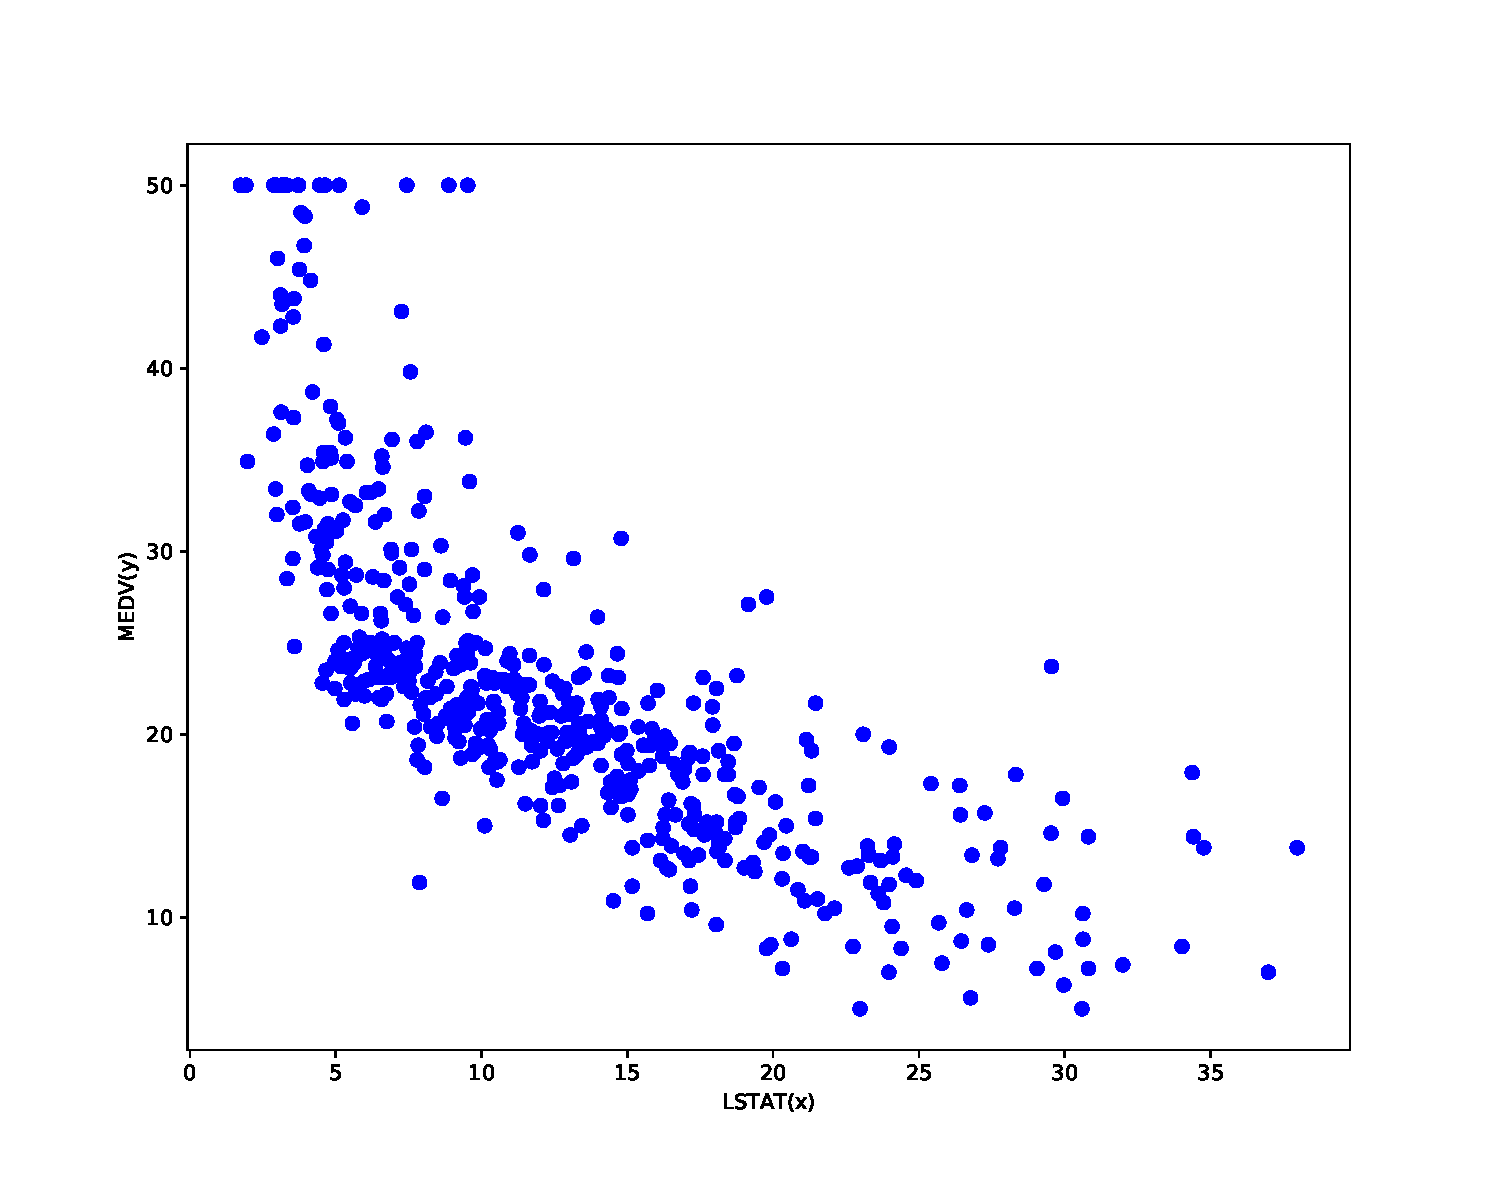
\includegraphics[width=8cm]{fig1.pdf}
	\caption{Scatter plot of training data}
	\label{fig:1}
\end{figure}
\begin{figure}[H]
	\centering 
	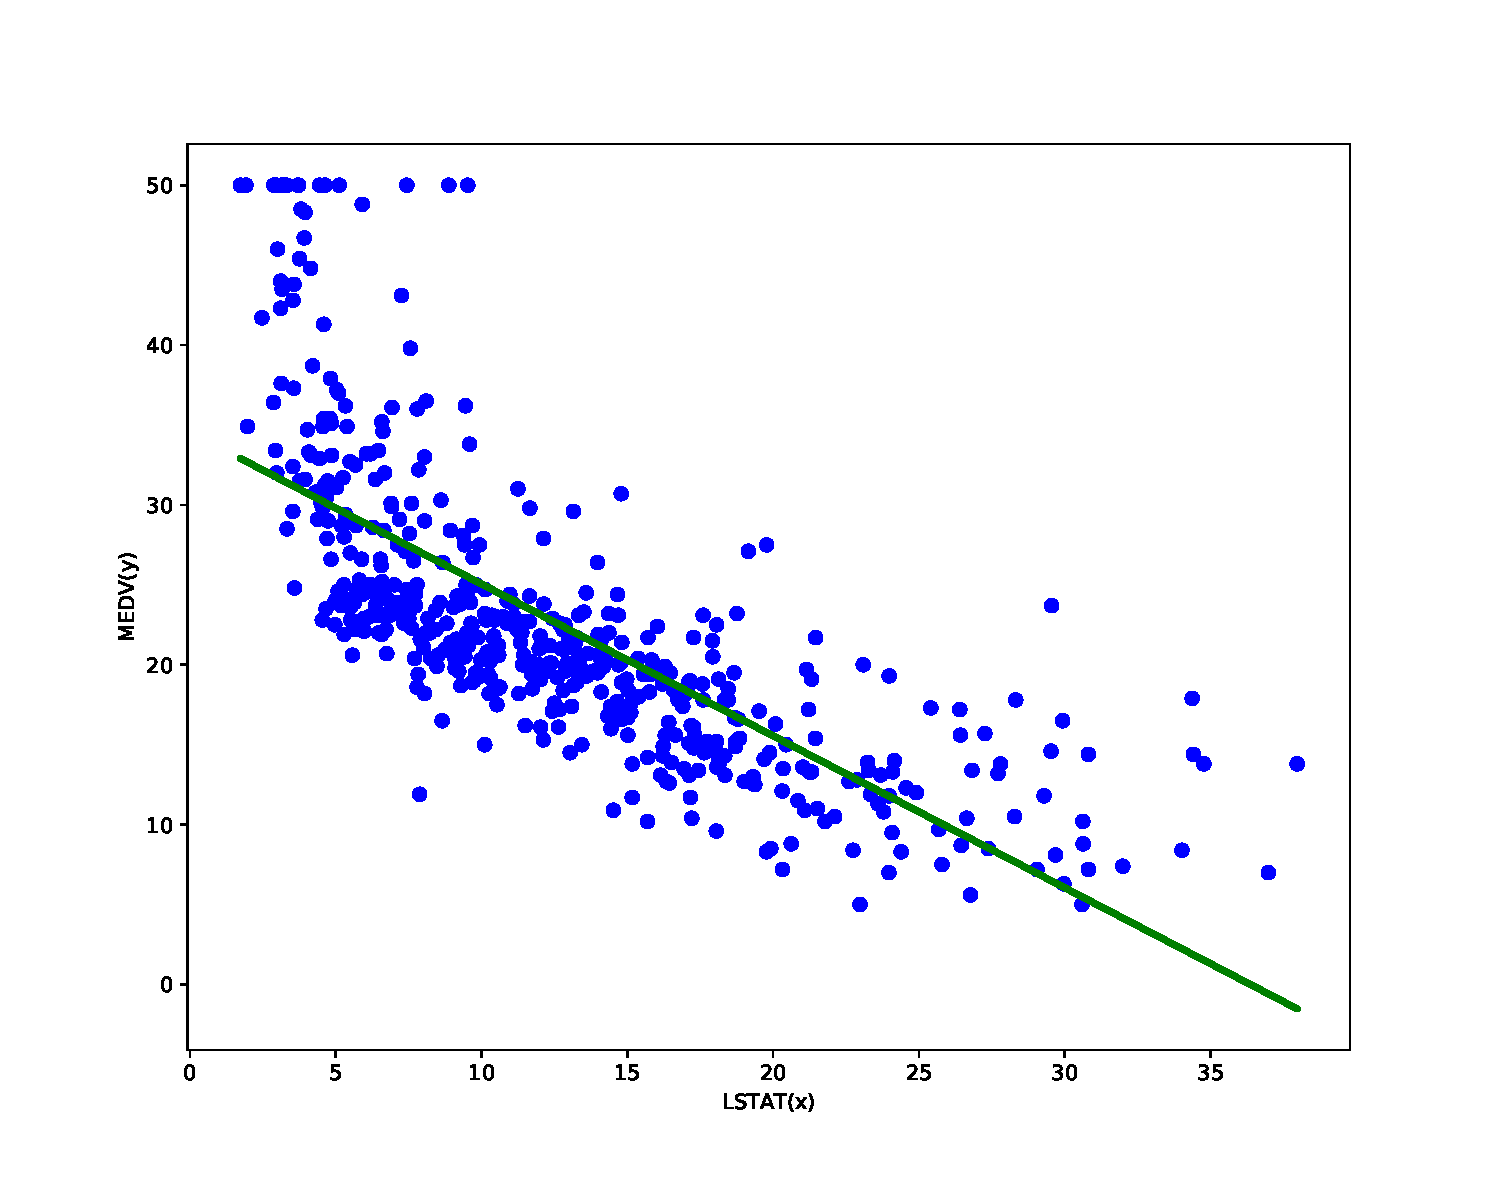
\includegraphics[width=8cm]{fig2a.pdf}
	\caption{Fitting a linear model to the data in Figure 1}
	\label{fig:2}
\end{figure}
\begin{figure}[H]
	\centering
	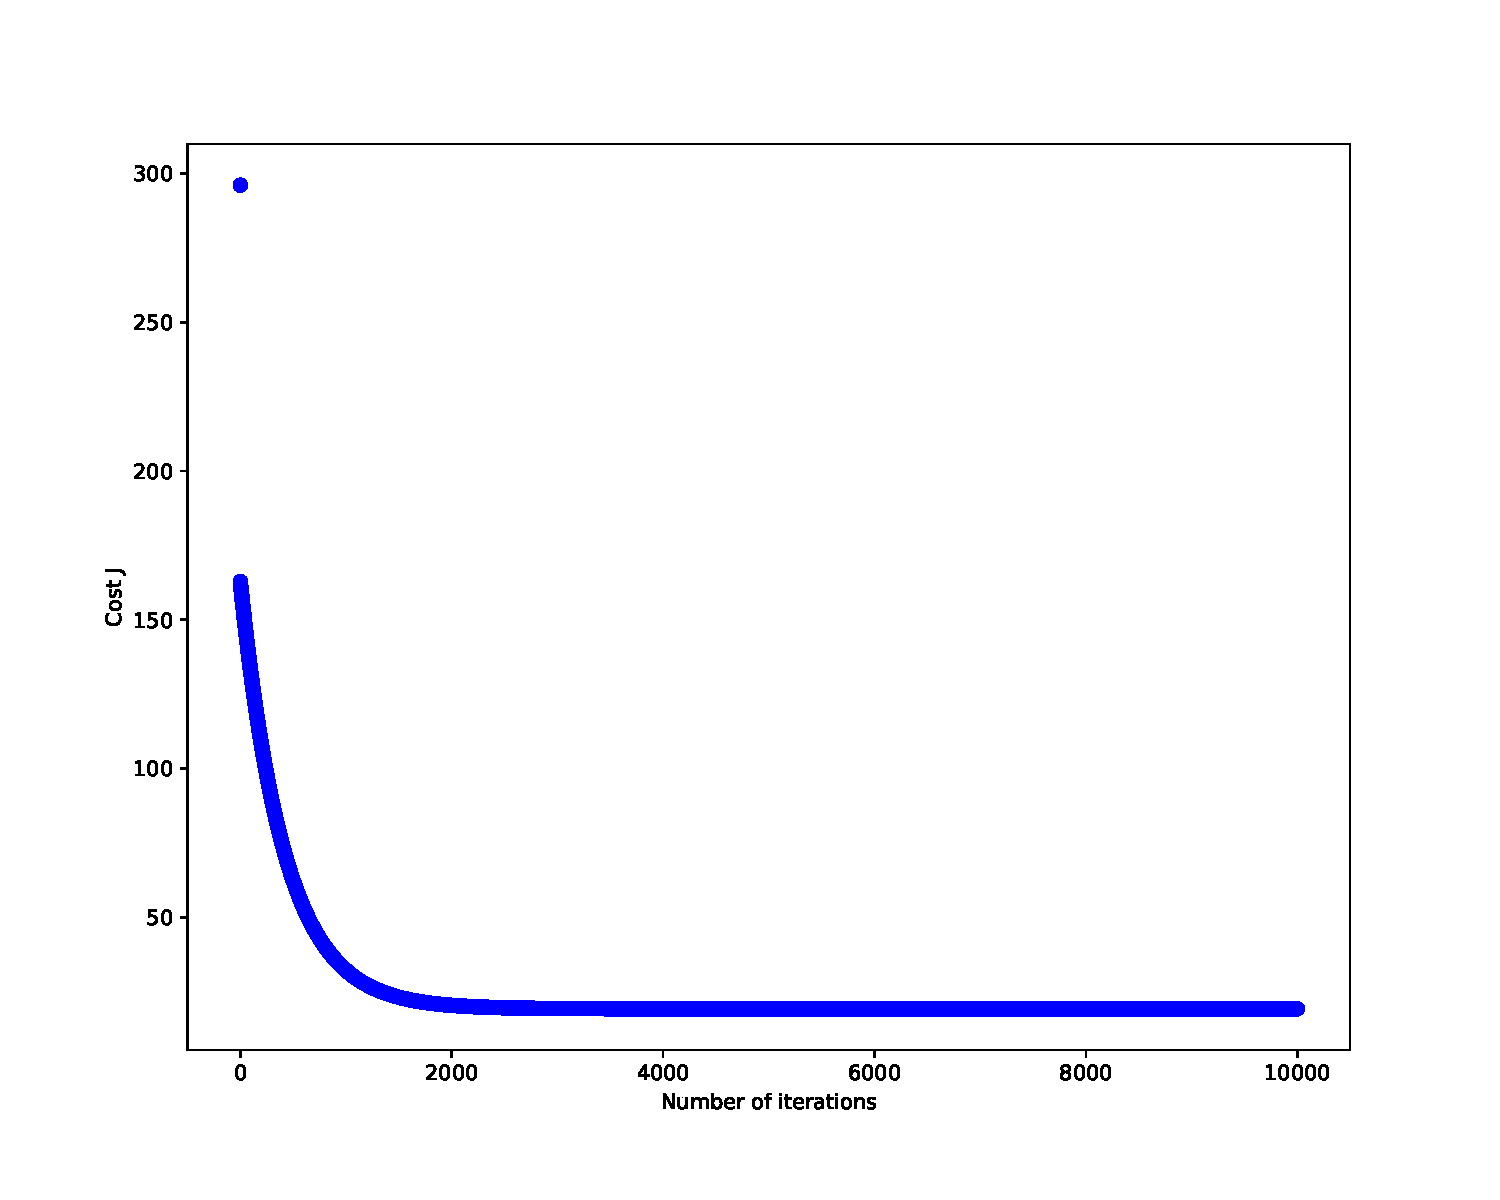
\includegraphics[width=8cm]{fig2b.pdf}
	\caption{Convergence of gradient descent to fit the linear model in Figure 2}
	\label{fig:3}
\end{figure}
\begin{enumerate}
	\item Qualitative analysis of the linear fit. What can you say about the quality of the linear fit for this data? In your assignment writeup.pdf, explain how you expect the model to perform at the low and high ends of values for LSTAT? How could we improve the quality of the fit?
	\begin{soln}
		As we can see in the Figure 2, the linear fit for this data is not that good, especially at the high and low ends. The regression should have some curve at the low and high ends of values for LSTAT, which We can replace x with some non-linear function to model non-linear relationship. Using polynomial regression. 
	\end{soln}
	
\end{enumerate}
\textbf{Problem 3.1.A3 Predicting on unseen data}
\begin{enumerate}
	\item Make predictions on median home values for census tracts where the percentage of the population of lower economic status is 5\% and 50\%.
	\begin{soln}
		For lower status percentage = 5, we predict a median home value of 298034.4941220727\\
		For lower status percentage = 50, we predict a median home value of -129482.12889798547
	\end{soln}
	\item Comparing with sklearn's linear regression model.
	\begin{soln} We can see from the data below that the results using different methods are quite similar.
		The coefficients computed by sklearn:  34.5538408794  and  -0.950049353758. \\
		The coefficients computed by gradient descent:  34.55363411 and -0.95003694.
		
		
	\end{soln}
	
\end{enumerate}
\textbf{Problem 3.1.B2 Loss function and gradient descent}\\
\begin{figure}[h]
	\centering
	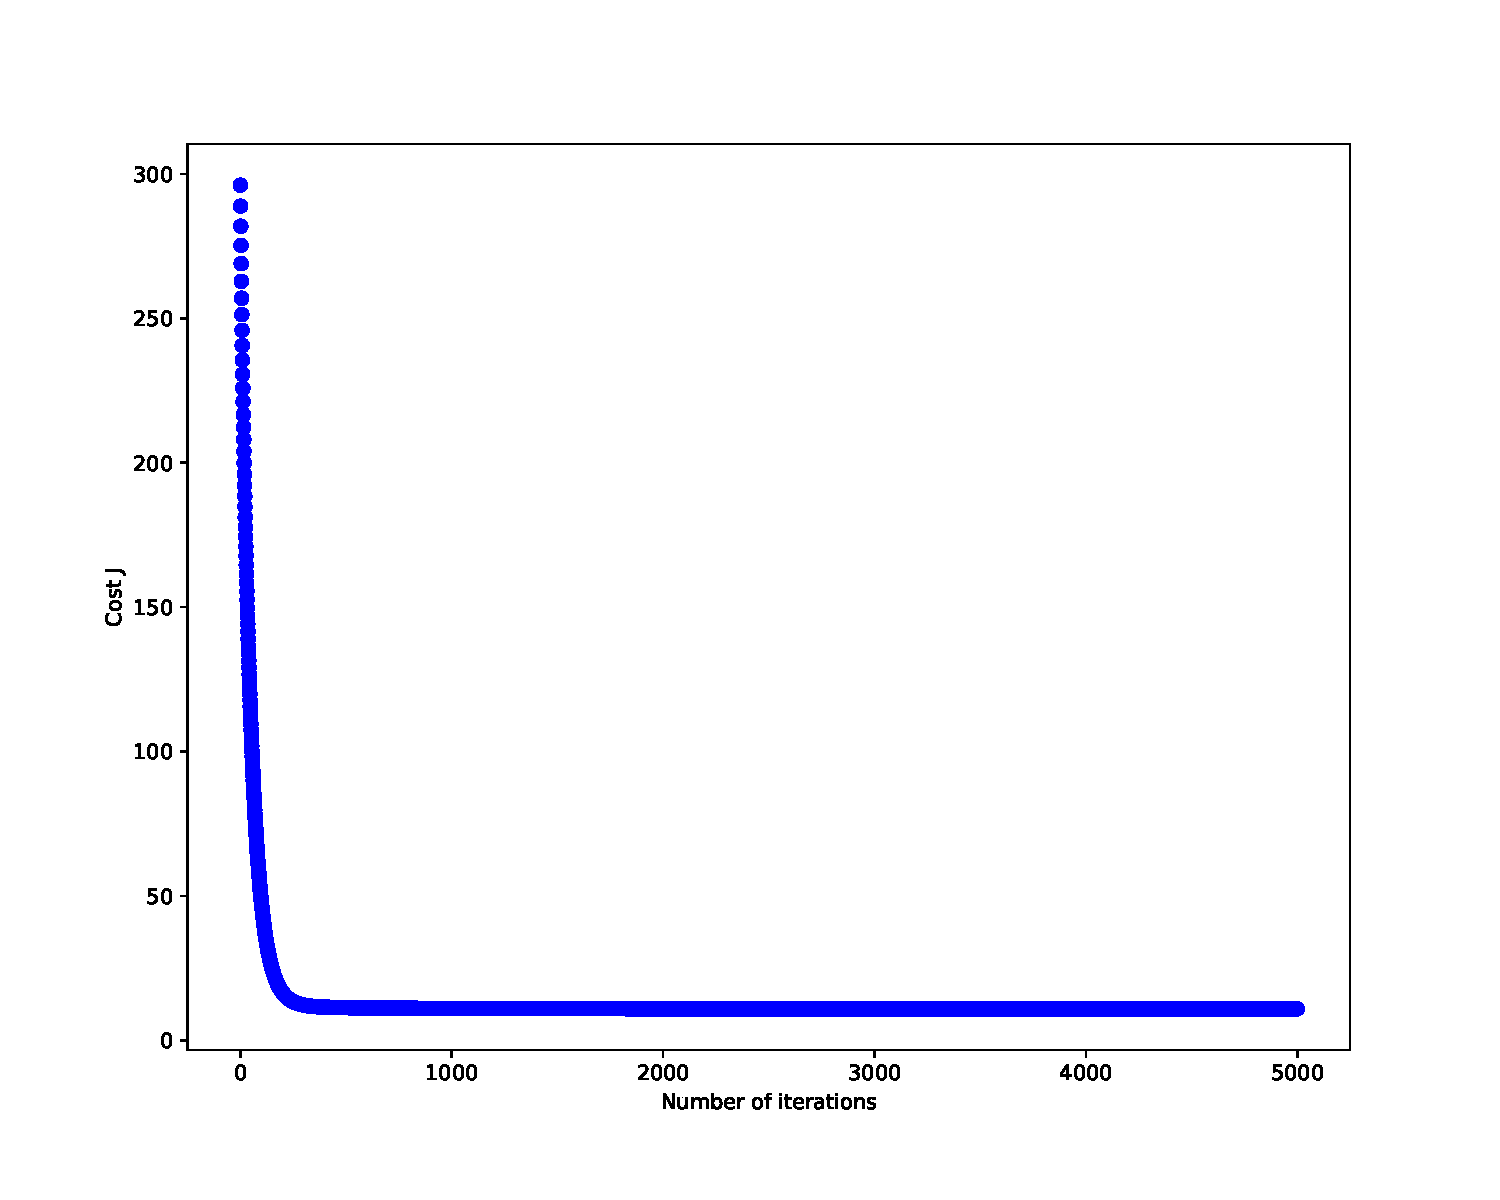
\includegraphics[width=7cm]{fig5.pdf}
	\caption{Number of iteration}
	\label{fig:4}
\end{figure}
\\
\textbf{Problem 3.1.B3 Predicting on unseen data}
\begin{flushleft}
	For average home in Boston suburbs, we predict a median home value of 225328.063241
\end{flushleft}
\textbf{Problem 3.1.B4: Normal equations (5 points)}
\begin{flushleft}
	For average home in Boston suburbs, we predict a median home value of 225328.06324113606. The prediction matches.
\end{flushleft}
\textbf{Problem 3.1.B5: Exploring convergence of gradient descent}
%\begin{figure}[h]
%	\centering
%	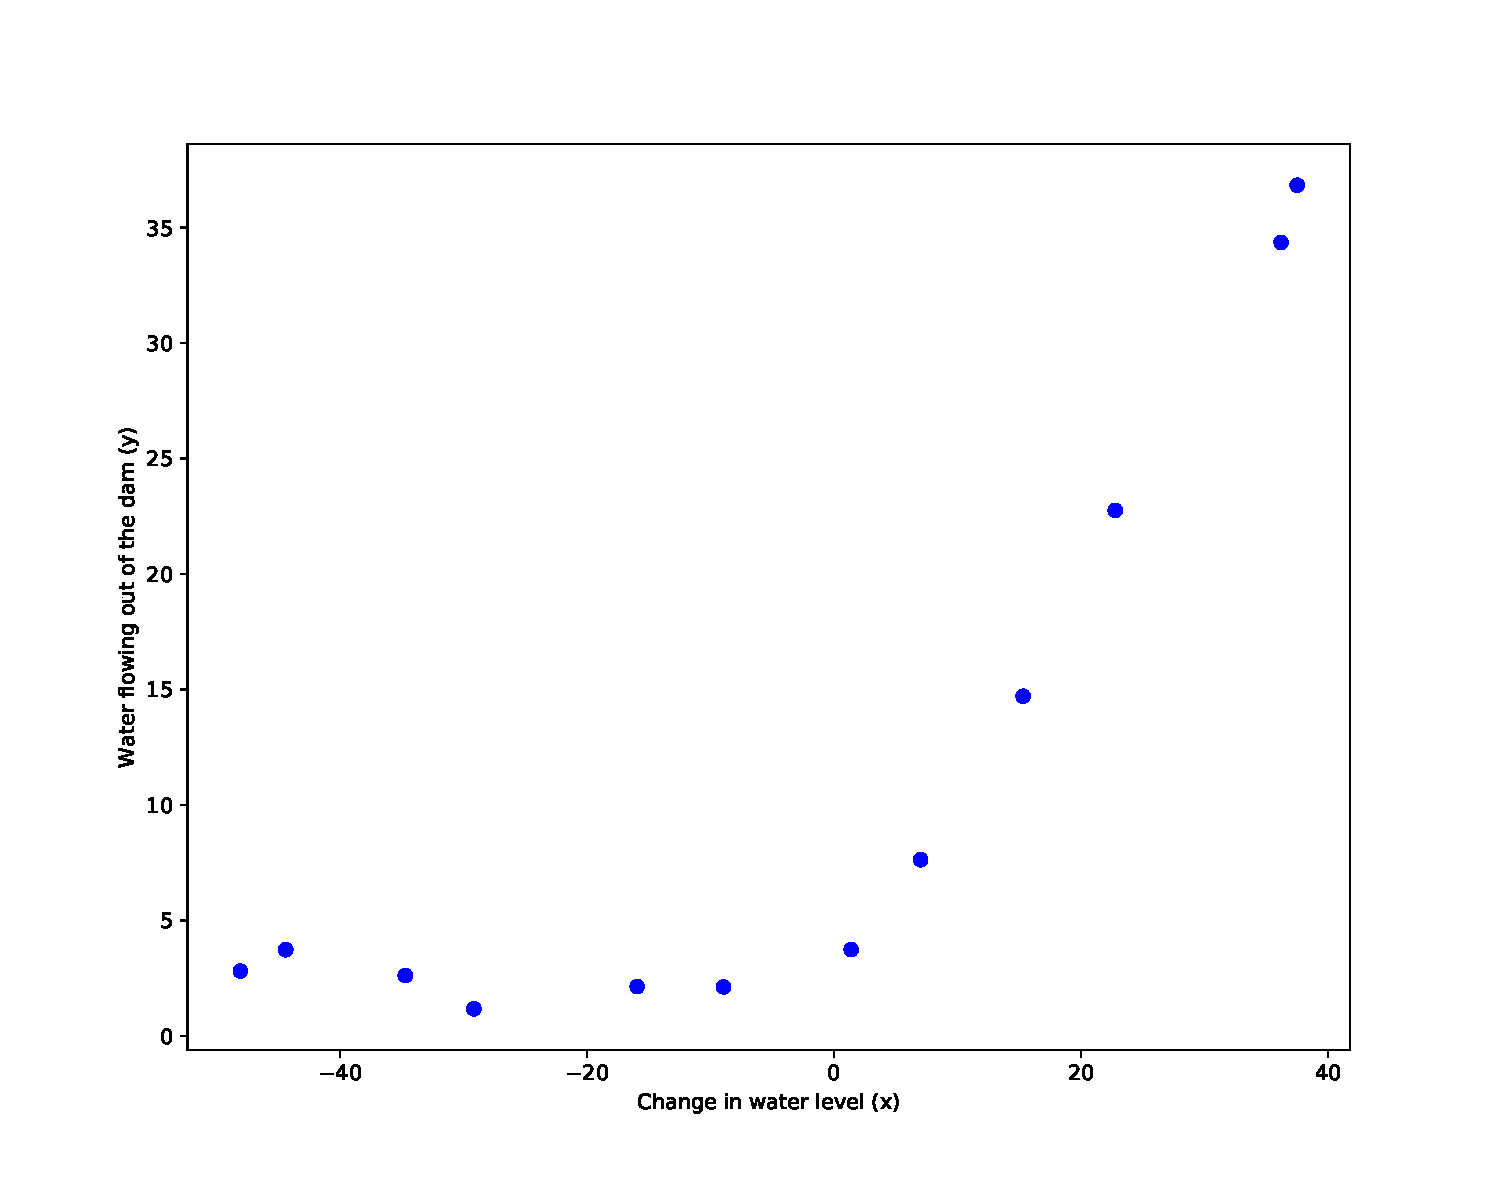
\includegraphics[width=8cm]{fig6.pdf}
%	\caption{Convergence of gradient descent for linear regression with multiple variables (Boston housing data set)}
%	\label{fig:5}
%\end{figure}
\begin{enumerate}
	\item Exploring convergence of gradient descent. What are good learning rates and number of iterations for this problem?
\begin{figure}[H]
	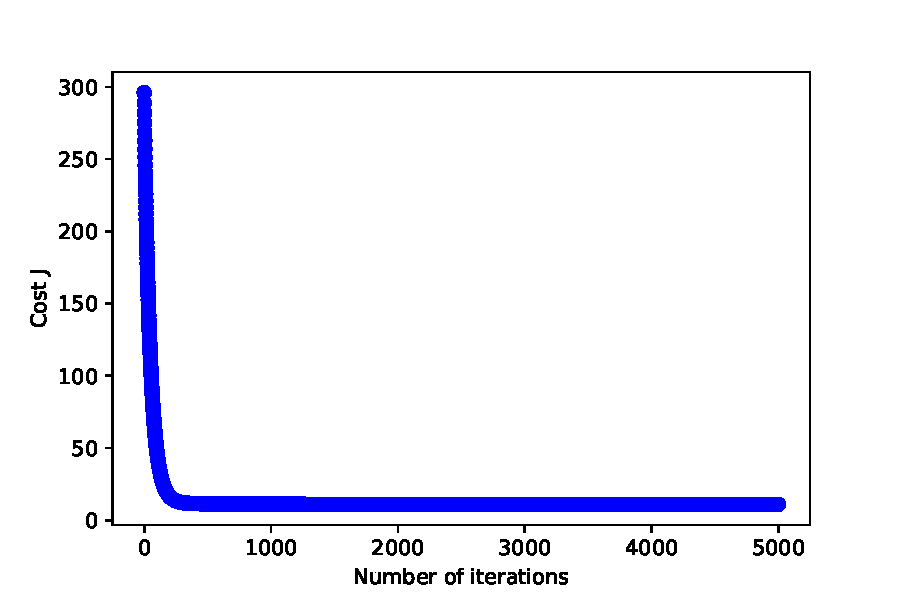
\includegraphics[width=6cm]{fig_0.01.pdf}
	\includegraphics[width=6cm]{fig_0.03pdf}
	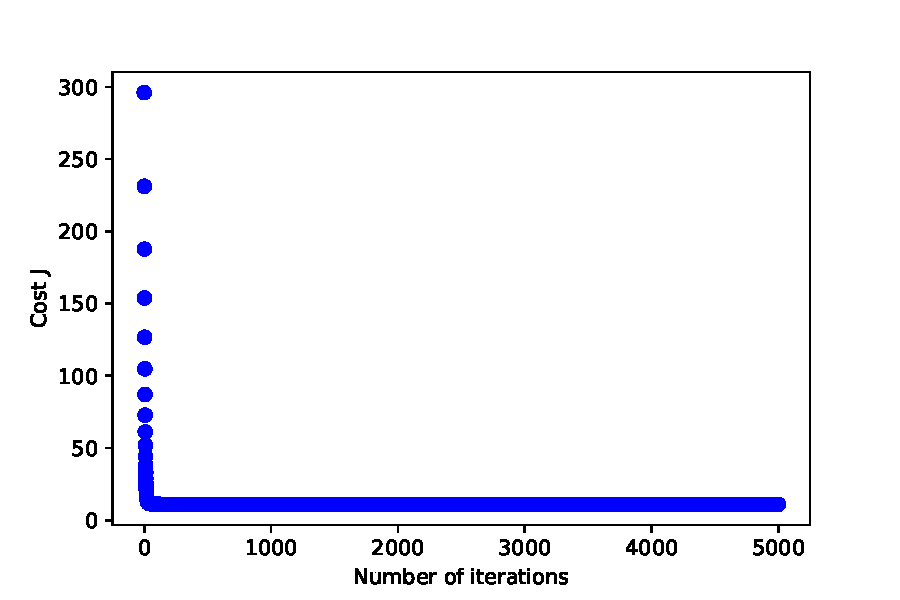
\includegraphics[width=6cm]{fig_0.1.pdf}
	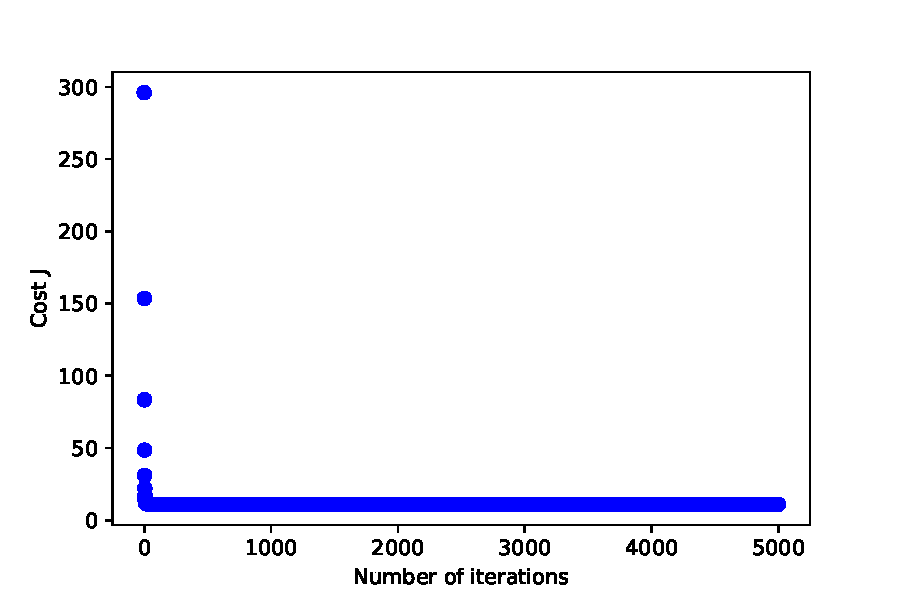
\includegraphics[width=6cm]{fig_0.3.pdf}
	\caption{Adjusting the regularization parameter}
	\label{fig:5}
\end{figure}		
\end{enumerate}
\textbf{Problem 3.2 Visualizing the dataset}
\begin{figure}[H]
	\centering
	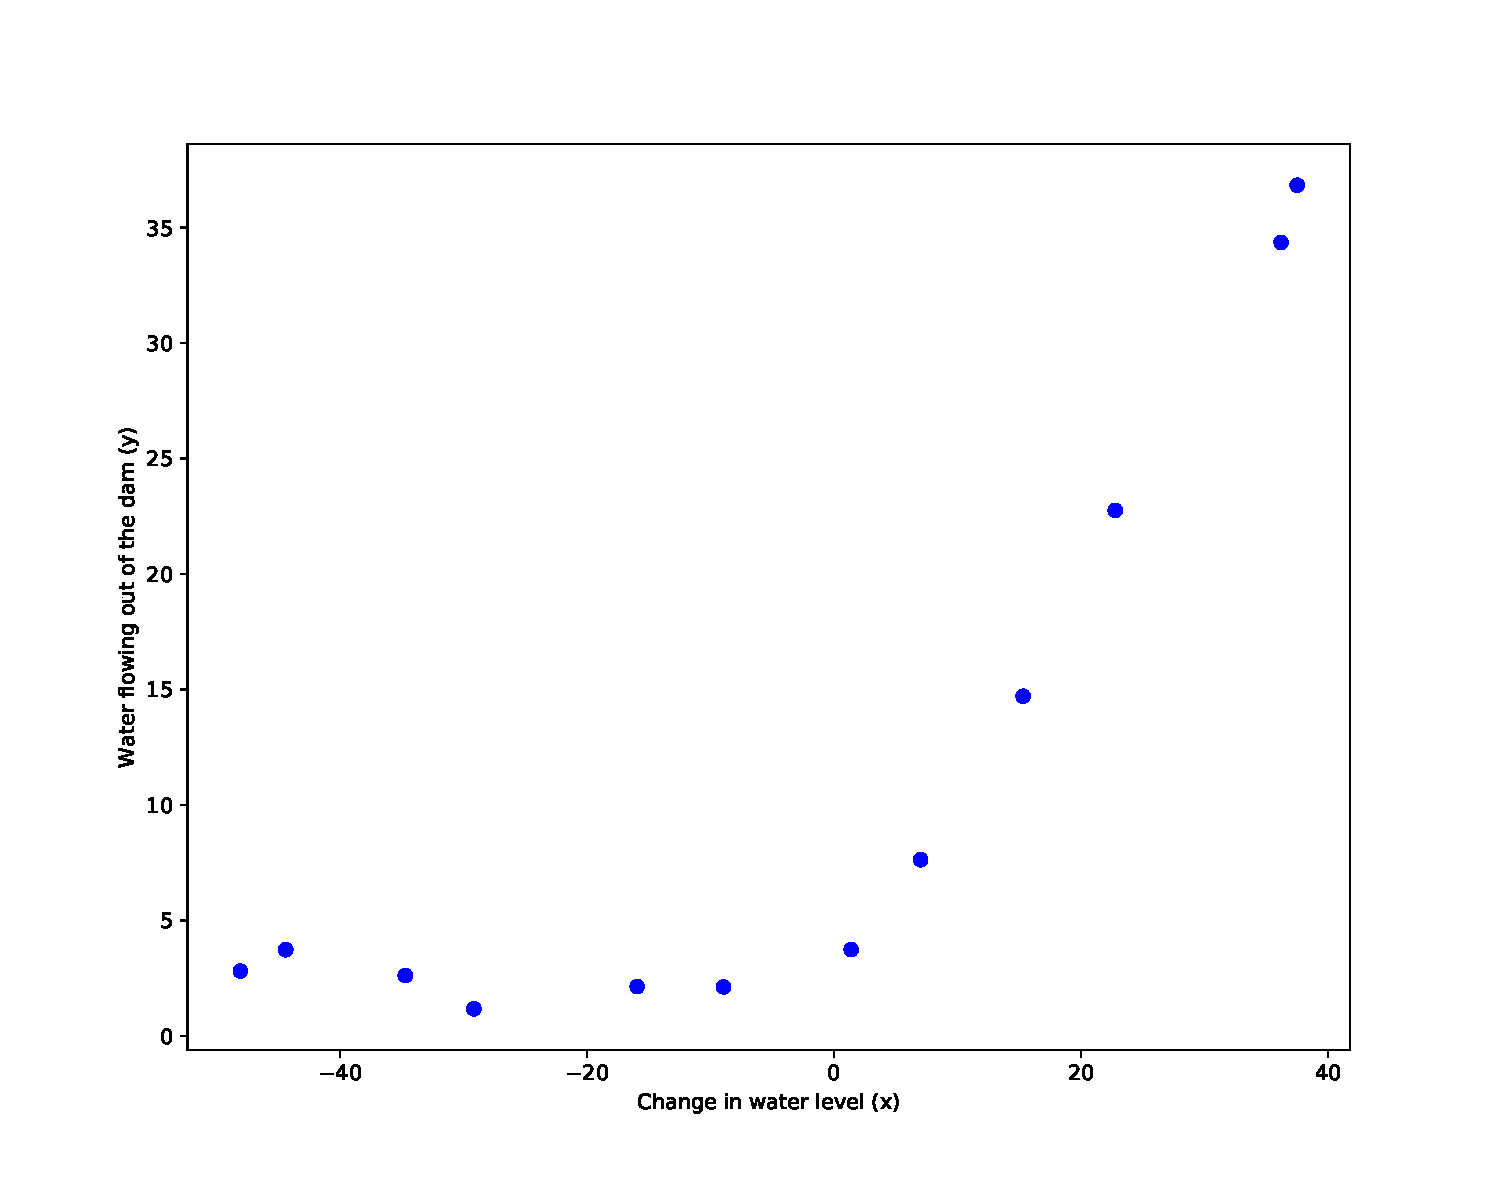
\includegraphics[width=8cm]{fig6.pdf}
	\caption{The training data for regularized linear regression}
	\label{fig:6}
\end{figure}

\textbf{Problem 3.2.A2 Regularized linear regression cost function}
\begin{figure}[H]
	\centering
	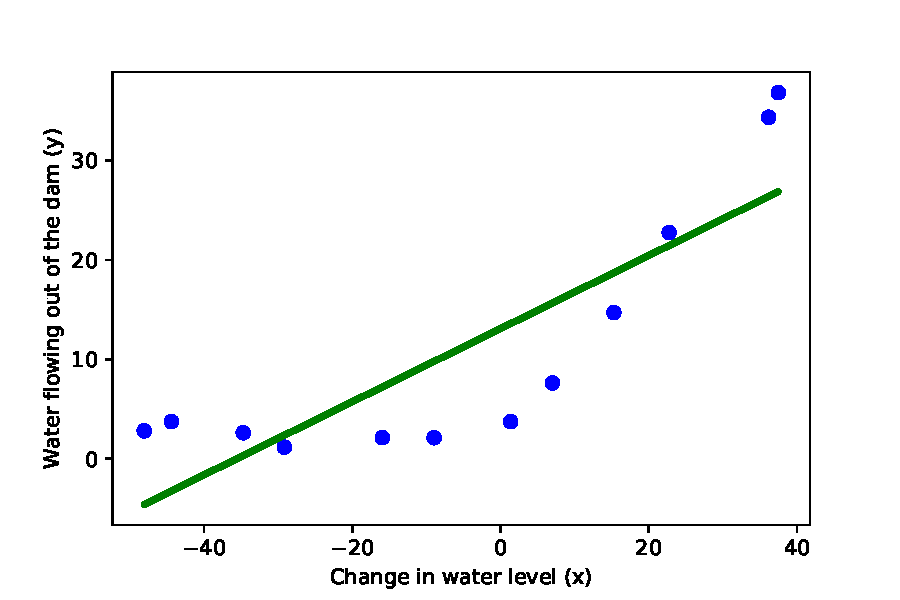
\includegraphics[width=8cm]{fig7.pdf}
	\caption{The best fit line for the training data}
	\label{fig:7}
\end{figure}

\textbf{Problem 3.2.A3 Learning curves}
\begin{figure}[H]
	\centering
	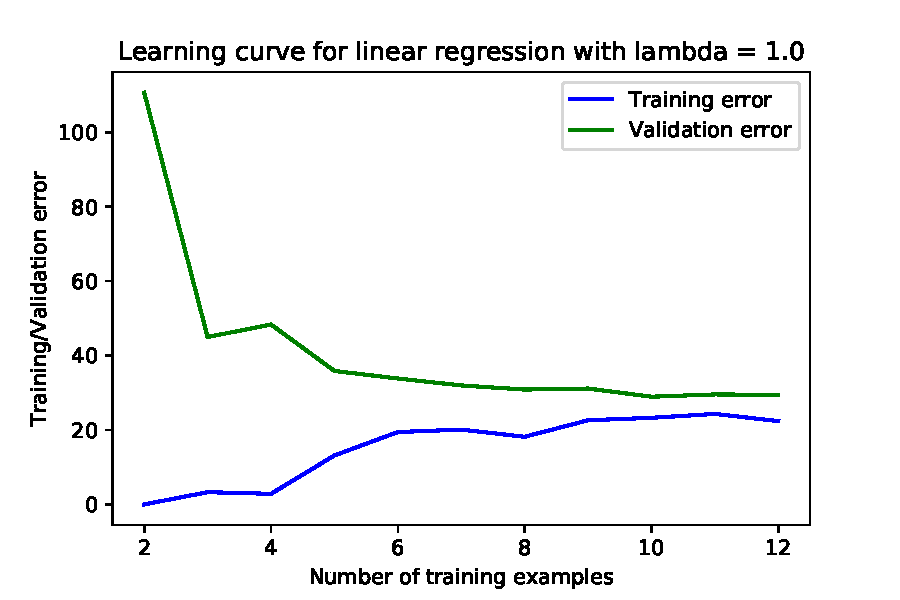
\includegraphics[width=8cm]{fig8.pdf}
	\caption{Learning curves}
	\label{fig:8}
\end{figure}

\textbf{Problem 3.2 Learning polynomial regression models}
\begin{figure}[H]
	\centering
	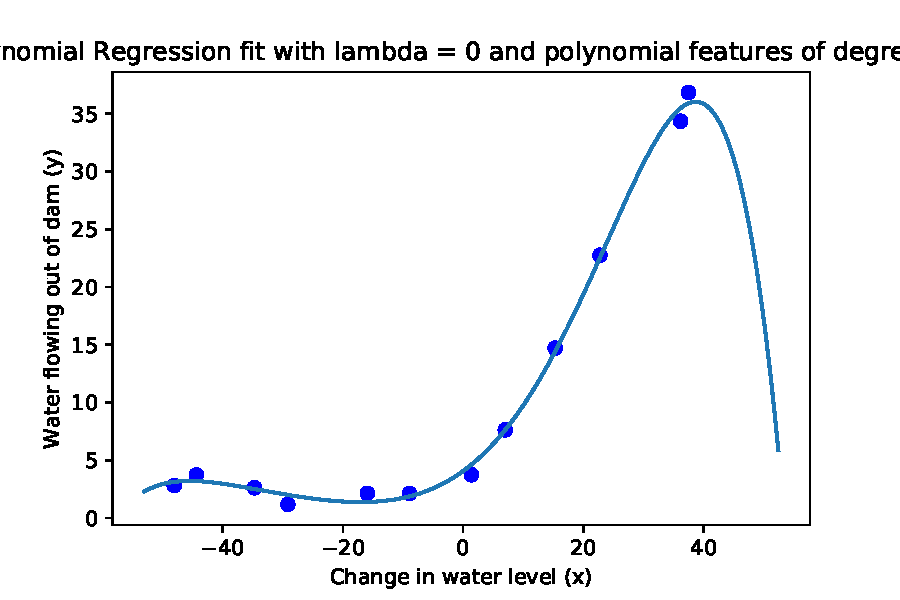
\includegraphics[width=8cm]{fig9.pdf}
	\caption{Polynomial fit for lambda = 0 with a p=6 order model.}
	\label{fig:9}
\end{figure}
\begin{figure}[H]
	\centering
	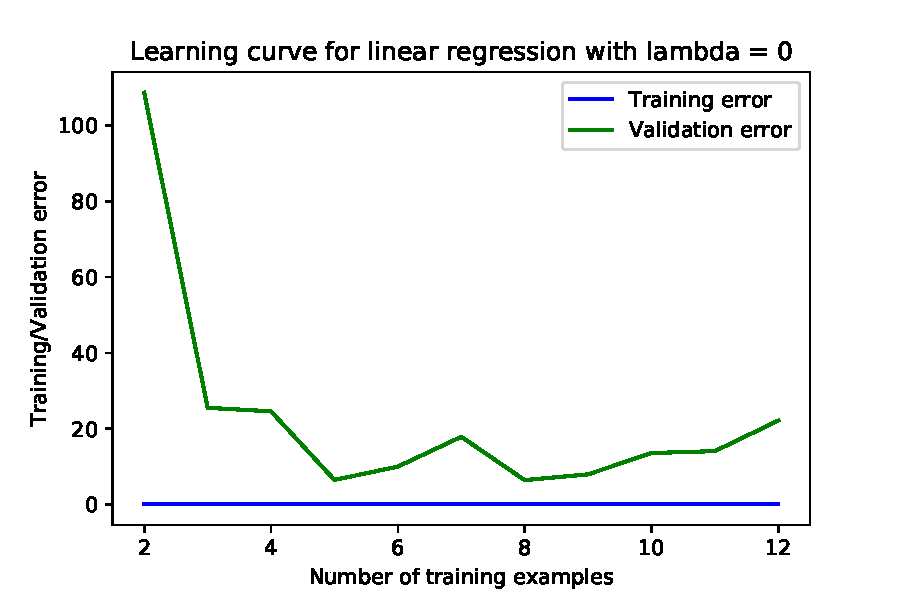
\includegraphics[width=8cm]{fig10.pdf}
	\caption{Learning curve for lambda = 0.}
	\label{fig:10}
\end{figure}
\textbf{Problem 3.2.A4: Adjusting the regularization parameter}
\begin{figure}[H]
	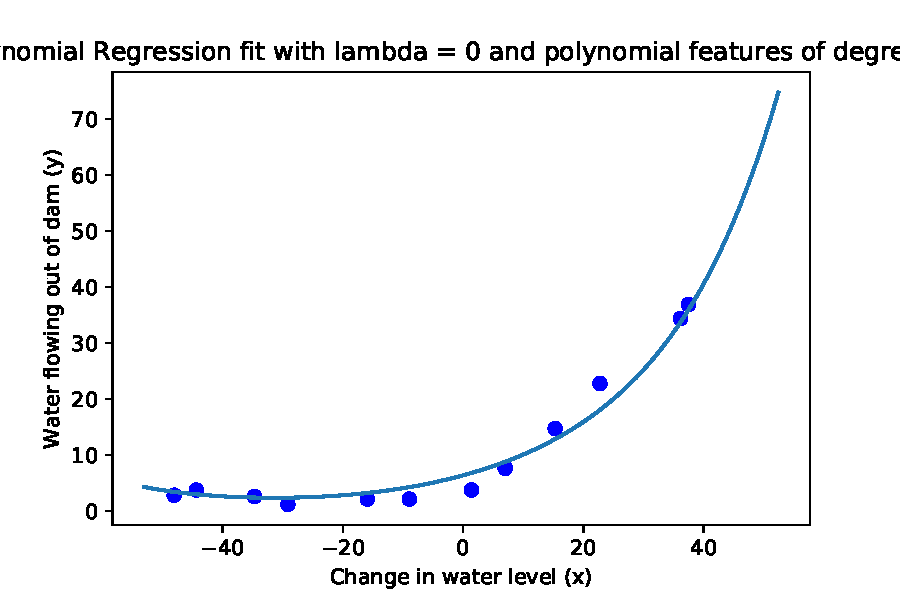
\includegraphics[width=5.5cm]{fig9_1.pdf}
	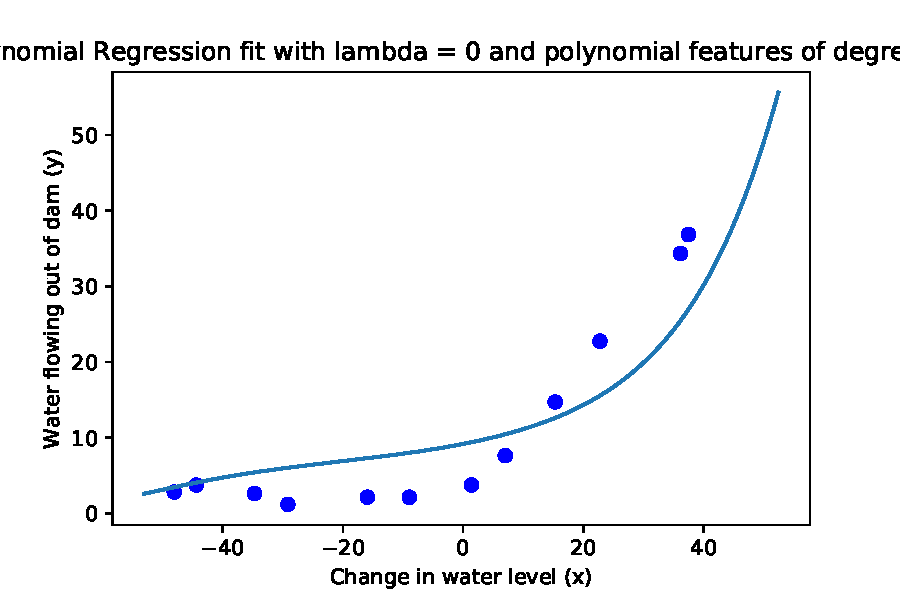
\includegraphics[width=5.5cm]{fig9_10.pdf}
	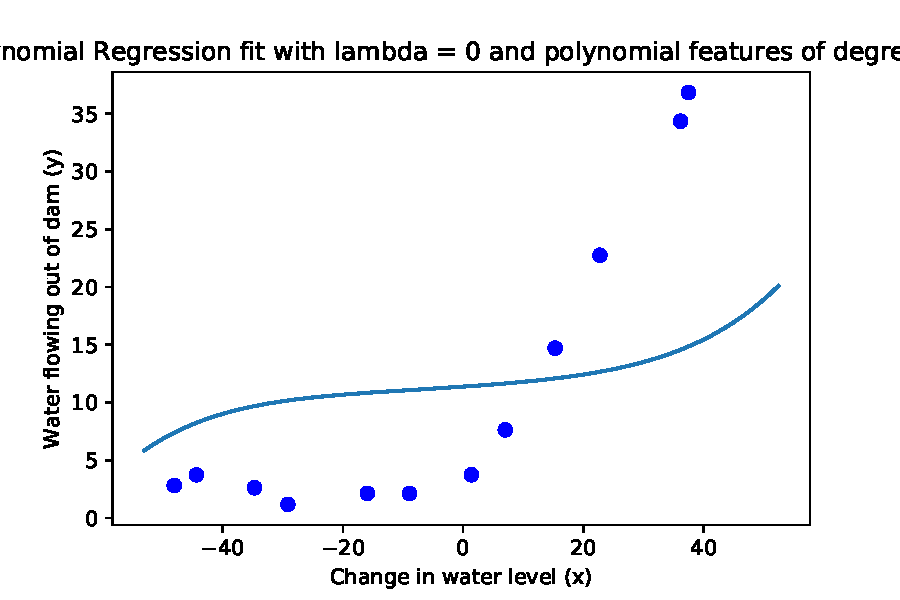
\includegraphics[width=5.5cm]{fig9_100.pdf}
	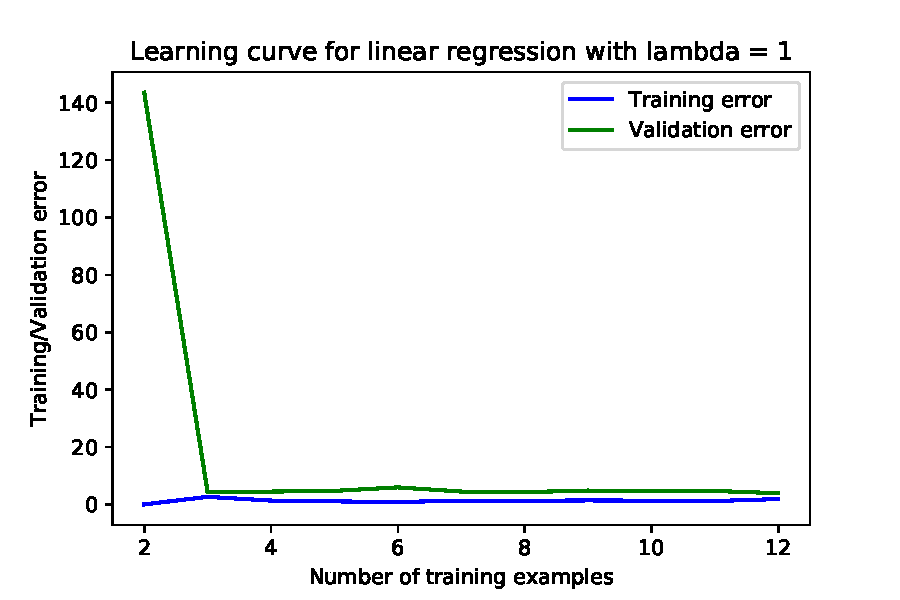
\includegraphics[width=5.5cm]{fig10_1.pdf}
	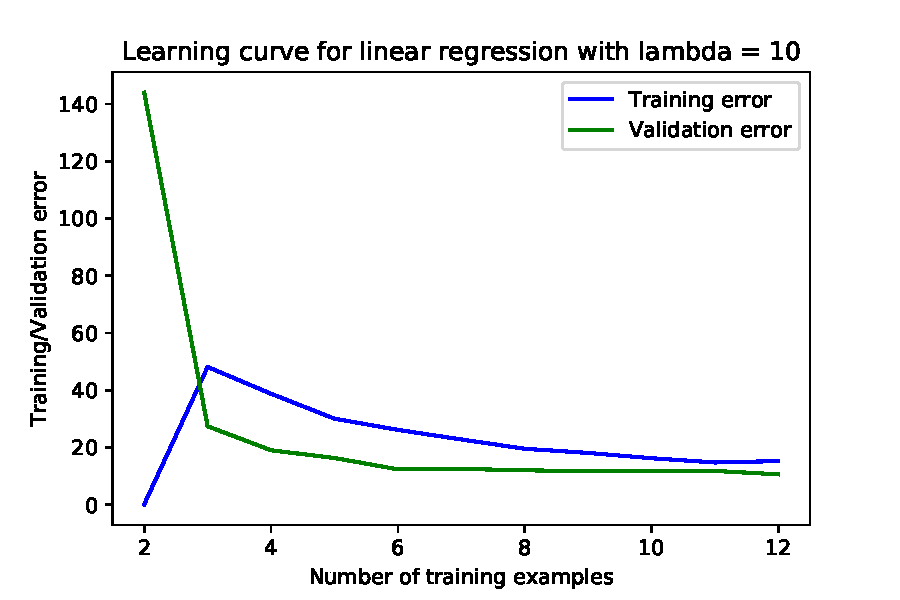
\includegraphics[width=5.5cm]{fig10_10.pdf}
	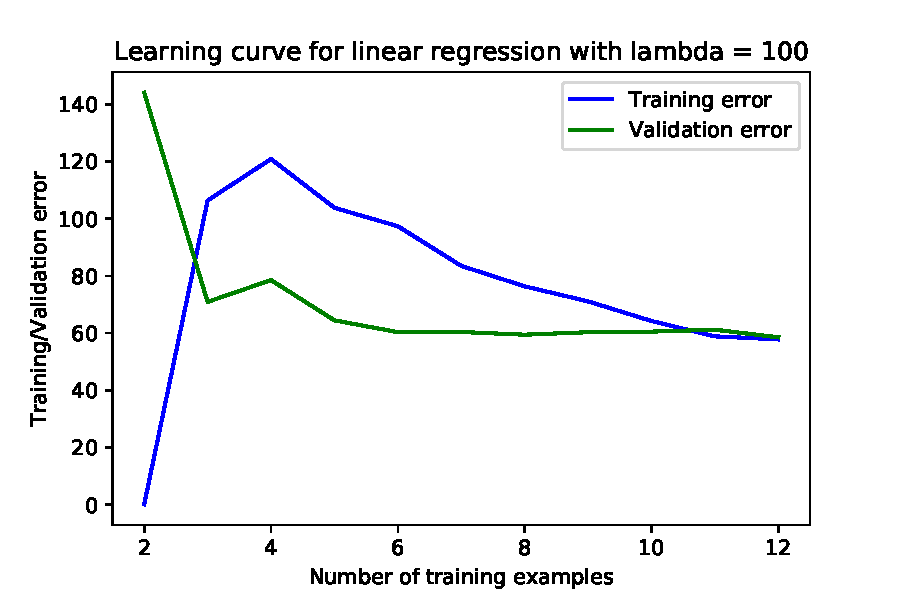
\includegraphics[width=5.5cm]{fig10_100.pdf}
	\caption{Adjusting the regularization parameter}
	\label{fig:11}
\end{figure}
\begin{flushleft}
	Increasing lambda results in less overfitting but also greater bias. The training error and testing error increase as long as the lambda increases.
\end{flushleft}
\textbf{Problem 3.2.A5: Selecting λ using a validation set}
\begin{figure}[H]
	\centering
	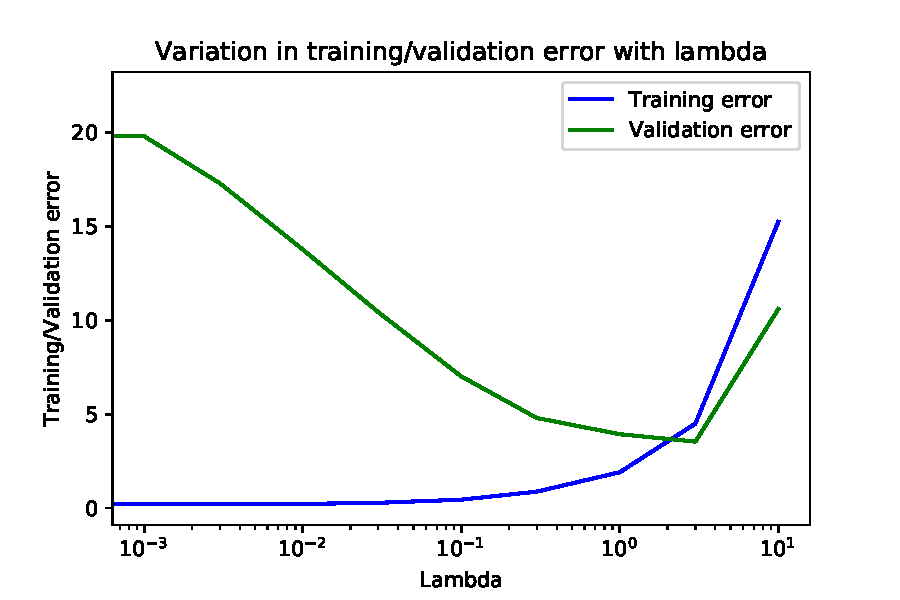
\includegraphics[width=8cm]{fig10to11.pdf}
	\caption{training and validation error on different lambda}
	\label{fig:12}
\end{figure}
\begin{flushleft}
	The best model is lambda = 3. When lambda = 3, the validation error is the smallest. 
\end{flushleft}
\textbf{Problem 3.2.A6: Computing test set error on the best model}
\begin{flushleft}
	When lambda = 0.3, the model has the smallest validation error. The test error is: 5.857077821089781
\end{flushleft}
\textbf{Problem 3.2.A7: Plotting learning curves with randomly selected examples}
\begin{figure}[H]
	\centering
	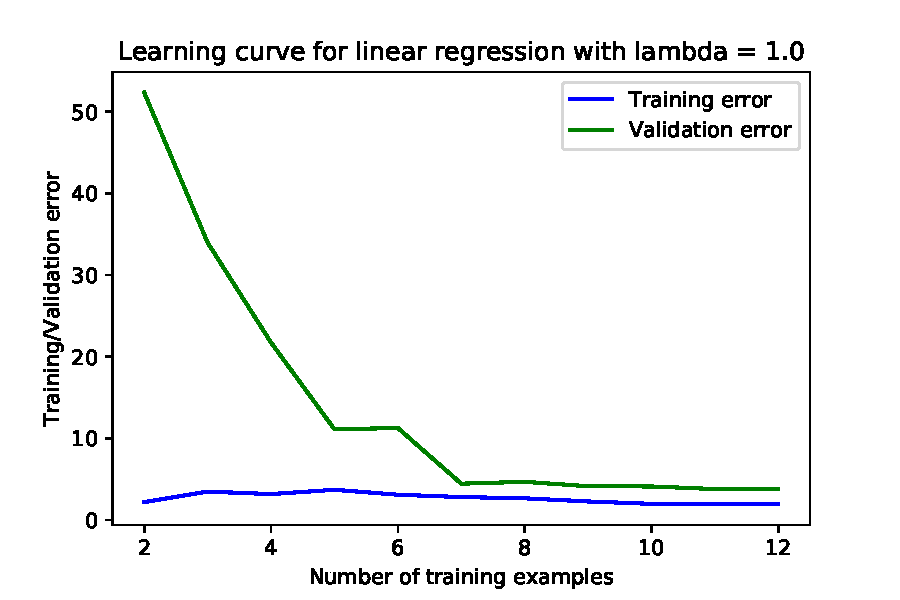
\includegraphics[width=8cm]{fig11.pdf}
	\caption{Averaged Learning curve for $lambda = 1$}
	\label{fig:13}
\end{figure}

\subsection*{Extra Credit: Building regularized models for Boston data set}
\begin{enumerate}
	\item Use sklearn's built-in functions to split the data into training, validation and test sets. 
	\begin{soln}
		I divide the data set into 3 different parts. The training set comes from 50\% of the data, the validation set comes from 25\% of the data, and the test set comes from 25\% of the data.
	\end{soln}
	\item What is the lowest achievable error on the test set with  $\lambda$ =0  ?
	\begin{soln}
		When $\lambda = 0$, the error of on the test set is 12.3122226194.
	\end{soln}
	\item Select the best value for  $\lambda$  and report the test set error with the best $\lambda$.
	\begin{soln}
		I select the value of $\lambda$ using validation set. The result is shown in figure \ref{fig:select_lambda_1}.
		\begin{figure}[H]
			\centering
			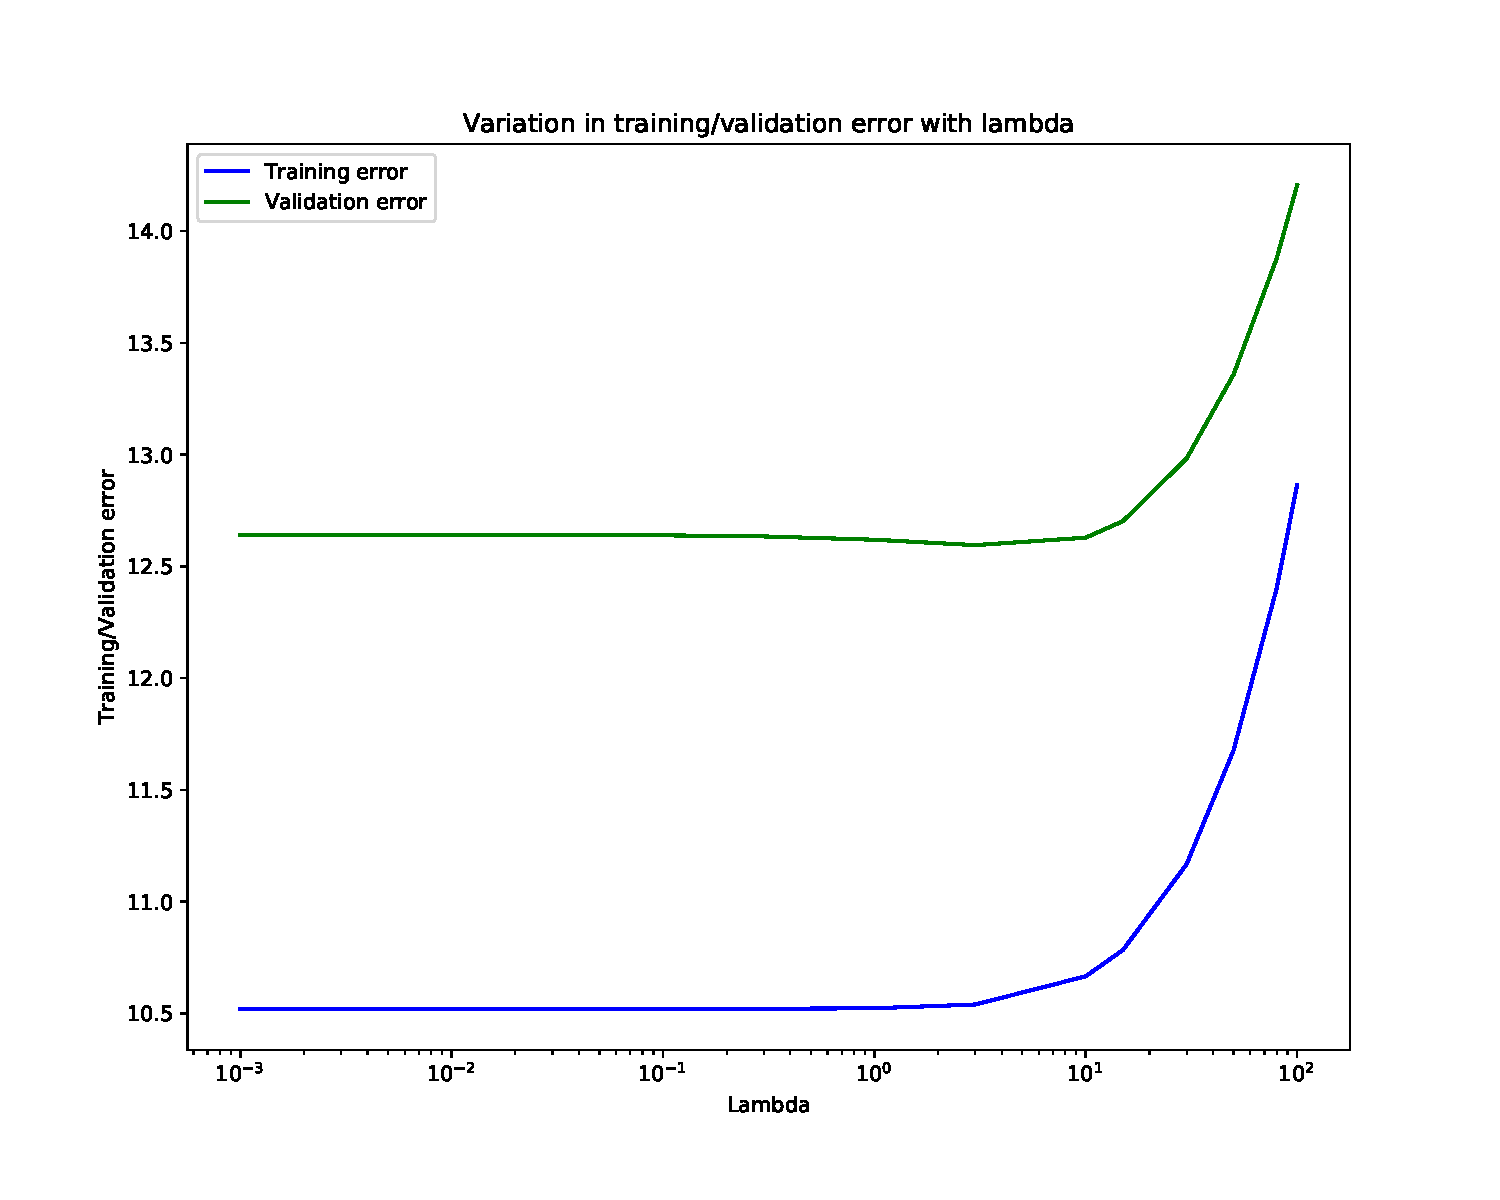
\includegraphics[width=8cm]{imgs//select_lambda_1.pdf}
			\caption{Select value for $\lambda$ using validation set}
			\label{fig:select_lambda_1}
		\end{figure}
	We can see that when $\lambda = 3$, the validation error is the lowest.
	\end{soln}
	\item Polynomial regression: quadratic features.
	\begin{soln}
		After transform data into polynomial, I repeated the steps above. At first I do $\lambda$ selection using validation set. The $\lambda$ selection result is shown in figure \ref{fig:select_lambda_2}
		\begin{figure}[H]
			\centering
			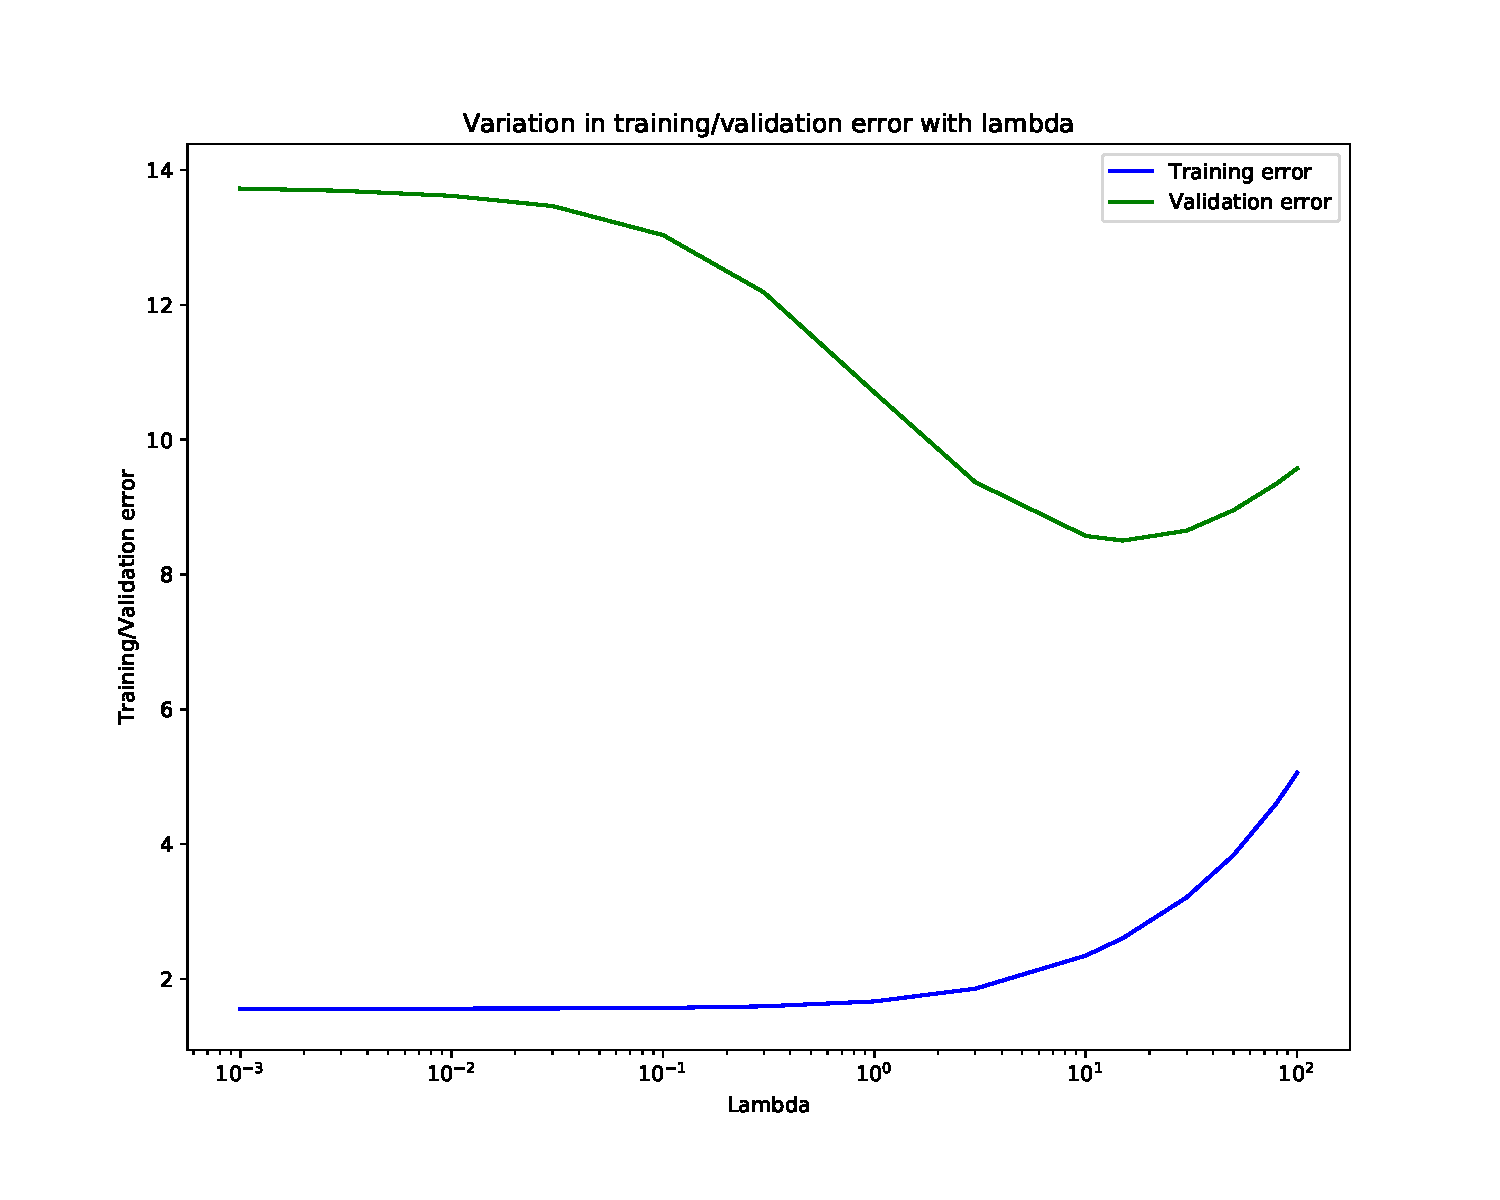
\includegraphics[width=8cm]{imgs//select_lambda_2.pdf}
			\caption{Select value for $\lambda$ using validation set for quadratic features}
			\label{fig:select_lambda_2}
		\end{figure}
		We select $\lambda = $. Then we train the model with $\lambda = $, the error is:7.09036691533.
	\end{soln}
	\item Polynomial regression: cubic features.
	\begin{soln}
		After transform data into polynomial, I repeated the steps above. At first I do $\lambda$ selection using validation set. The $\lambda$ selection result is shown in figure \ref{fig:select_lambda_3}
		\begin{figure}[H]
			\centering
			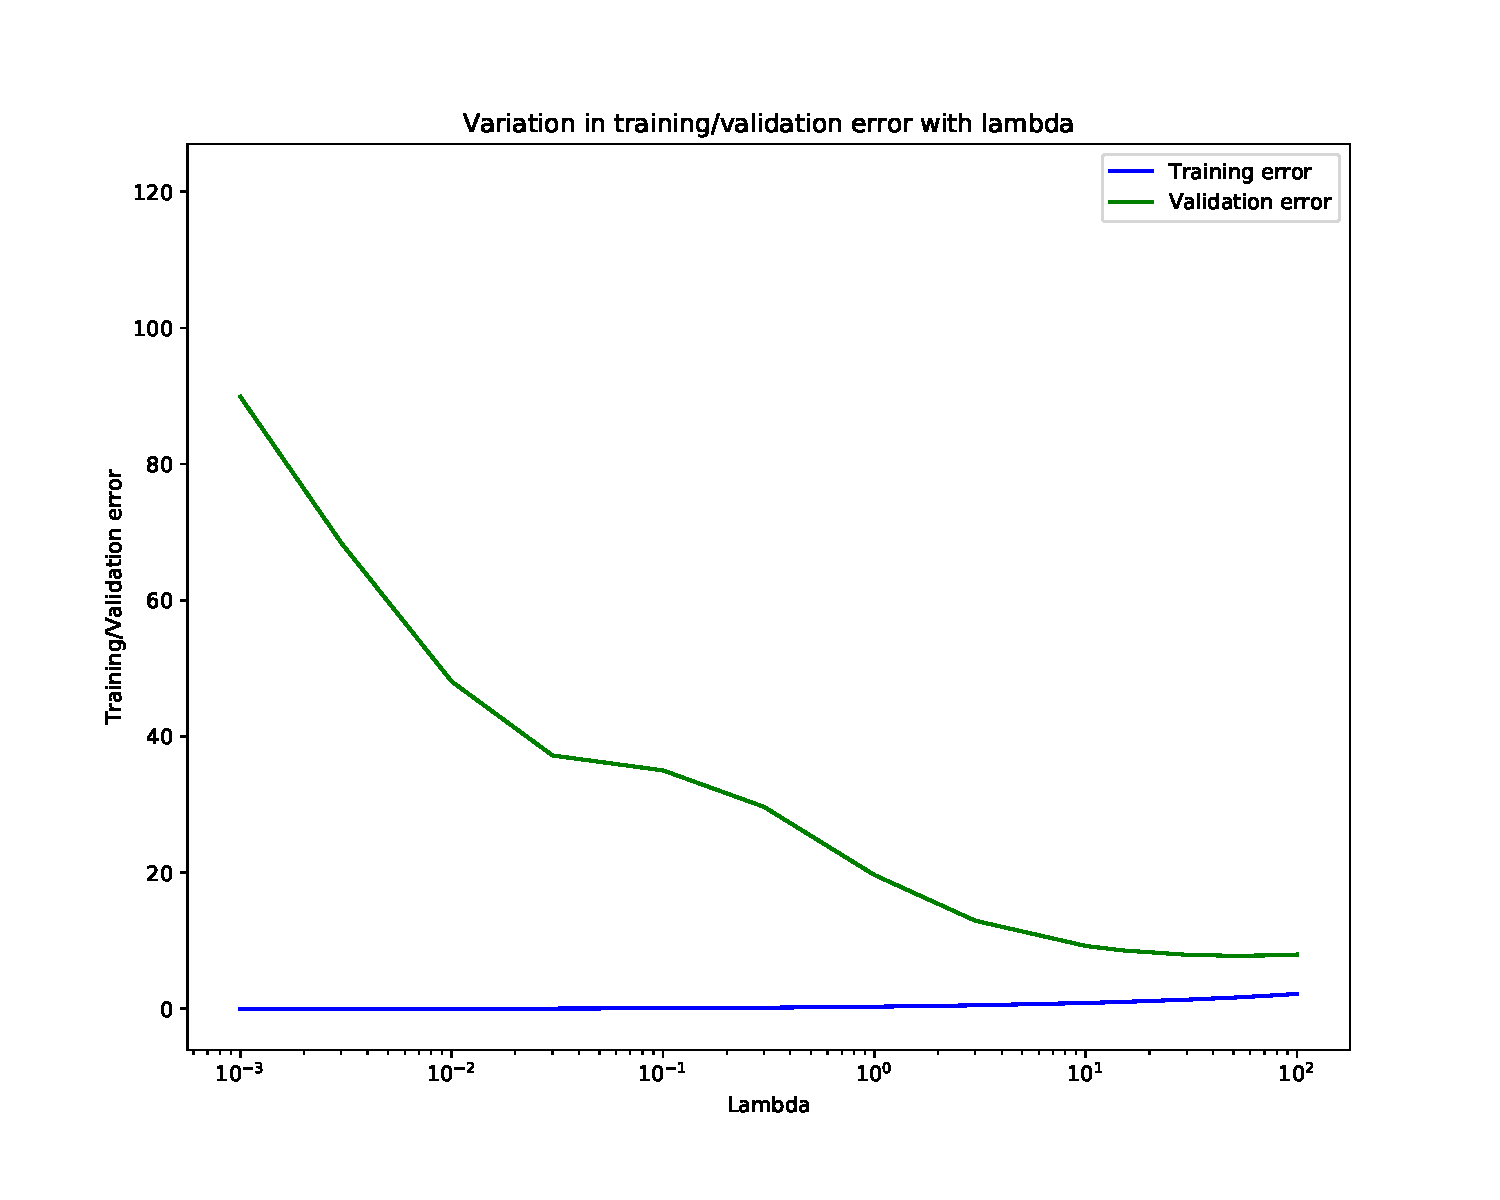
\includegraphics[width=8cm]{imgs//select_lambda_3.pdf}
			\caption{Select value for $\lambda$ using validation set for cubic features}
			\label{fig:select_lambda_3}
		\end{figure}
		We select $\lambda = 10$. Then we train the model with $\lambda = 10$, the error is:7.09036691533.
	\end{soln}
\end{enumerate}





\end{document}


